%% 
%% Copyright 2007-2020 Elsevier Ltd
%% 
%% This file is part of the 'Elsarticle Bundle'.
%% ---------------------------------------------
%% 
%% It may be distributed under the conditions of the LaTeX Project Public
%% License, either version 1.2 of this license or (at your option) any    
%% later version.  The latest version of this license is in
%%    http://www.latex-project.org/lppl.txt
%% and version 1.2 or later is part of all distributions of LaTeX
%% version 1999/12/01 or later.
%% 
%% The list of all files belonging to the 'Elsarticle Bundle' is
%% given in the file `manifest.txt'.
%% 
%% Template article for Elsevier's document class `elsarticle'
%% with harvard style bibliographic references

\documentclass[preprint,12pt]{elsarticle}

%% Use the option review to obtain double line spacing
%% \documentclass[preprint,review,12pt]{elsarticle}

%% Use the options 1p,twocolumn; 3p; 3p,twocolumn; 5p; or 5p,twocolumn
%% for a journal layout:
%% \documentclass[final,1p,times]{elsarticle}
%% \documentclass[final,1p,times,twocolumn]{elsarticle}
%% \documentclass[final,3p,times]{elsarticle}
%% \documentclass[final,3p,times,twocolumn]{elsarticle}
%% \documentclass[final,5p,times]{elsarticle}
%% \documentclass[final,5p,times,twocolumn]{elsarticle}

%% For including figures, graphicx.sty has been loaded in
%% elsarticle.cls. If you prefer to use the old commands
%% please give \usepackage{epsfig}

%% The amssymb package provides various useful mathematical symbols
\usepackage{amssymb}
%% The amsthm package provides extended theorem environments
%% \usepackage{amsthm}

%% The lineno packages adds line numbers. Start line numbering with
%% \begin{linenumbers}, end it with \end{linenumbers}. Or switch it on
%% for the whole article with \linenumbers.
%% \usepackage{lineno}



\voffset=-1.5cm \hoffset=-1.4cm \textwidth=16cm \textheight=22.0cm
\usepackage[activate={true,nocompatibility},final,tracking=true,kerning=true,spacing=true,factor=1100,stretch=10,shrink=10]{microtype}
\hbadness=99999
\hfuzz=999pt 
\sloppy
\usepackage[utf8]{inputenc}
\usepackage[T1]{fontenc}
\usepackage{babel}

%\RequirePackage[sort&compress,numbers]{natbib}

%\bibliographystyle{config/bibstyle}

\renewcommand{\bibfont}{\small}
\usepackage{graphicx,color}
\usepackage{amsmath}
\usepackage[version=4]{mhchem}
\usepackage{siunitx}
\usepackage{longtable,tabularx}
\setlength\LTleft{0pt} 
\usepackage{subcaption}
\usepackage{hyperref}
\usepackage{ragged2e}
\usepackage{arydshln}
\usepackage{optidef} % to write optimization problems
\usepackage[ruled,vlined]{algorithm2e}  % to write algorithms
\usepackage{mathrsfs}   % to write cursive letters
\usepackage{changepage}   % to prevent overfull box
\usepackage{float} 
\usepackage{dsfont}
\usepackage{nccmath}
\usepackage{tabularx}
\usepackage{booktabs}
\usepackage{longtable}
\usepackage{enumitem}
\usepackage{adjustbox}
\usepackage{amsmath}               
\usepackage{amsfonts}               
\usepackage{stanli}
% New command to refer to equations as Eq.(1), Eq.(2), ...
\newcommand{\eqnref}[1]{Eq.~(\ref{#1})}
% New command to refer to figures as Fig.1, Fig.2, ...
\newcommand{\figref}[1]{Fig.~\ref{#1}}
\renewcommand{\figurename}{Fig.}
% New command to refer to tables as Tab.1, Tab.2, ...
\newcommand{\tabref}[1]{Table~\ref{#1}}
% New command to refer to algorithms as Alg.1, Alg.2, ...
\newcommand{\algref}[1]{Alg.~\ref{#1}}

\newcommand*\samethanks[1][\value{footnote}]{\footnotemark[#1]}

\usepackage{bm}

\usepackage{optidef} % to write optimization problems
\usepackage[ruled,vlined]{algorithm2e}  % to write algorithms
\usepackage{mathrsfs}   % to write cursive letters
\usepackage{changepage}   % to prevent overfull box
\usepackage{float} 
\usepackage{dsfont}
\let\openbox\relax
\usepackage{amsthm}
\usepackage{relsize}

\usepackage{nomencl}
\usepackage{multicol}
\setlength\columnsep{1cm}
\renewcommand{\nompreamble}{\begin{center}\begin{multicols}{2}}
\renewcommand{\nompostamble}{\end{multicols}\end{center}}
\setlength{\nomlabelwidth}{-0.1cm}
\setlength{\nomitemsep}{-0.15\parsep}
\makenomenclature
\providetoggle{nomsort}
\settoggle{nomsort}{true} % true = sort by use, false = sort as usual
\makeatletter
\iftoggle{nomsort}{%
    \let\old@@@nomenclature=\@@@nomenclature        
        \newcounter{@nomcount} \setcounter{@nomcount}{0}%
        \renewcommand\the@nomcount{\two@digits{\value{@nomcount}}}% Ensure 10>01
        \def\@@@nomenclature[#1]#2#3{% Taken from package documentation
          \addtocounter{@nomcount}{1}%
        \def\@tempa{#2}\def\@tempb{#3}%
          \protected@write\@nomenclaturefile{}%
          {\string\nomenclatureentry{\the@nomcount\nom@verb\@tempa @[{\nom@verb\@tempa}]%
          \begingroup\nom@verb\@tempb\protect\nomeqref{\theequation}%
          |nompageref}{\thepage}}%
          \endgroup
          \@esphack}%
      }{}
\makeatother      

\def\abs#1{\left\lvert#1\right\rvert}

\usepackage{xpatch}
\makeatletter
\xpatchcmd\SetKwInOut
  {\hangafter=1\parbox[t]}
  {\hangafter=1\justify\parbox[t]}
  {}{\fail}
\makeatother

\SetKwInOut{Input}{Input}
\DontPrintSemicolon

%to comment some large parts
\usepackage{comment}

 \def\emailname{E-mail}%
\def\email#1{\emailname: #1}
 \def\keywordname{{\bfseries Keywords}}%
  \def\andname{and}%
%remove when submitting:
%\usepackage{showlabels}
\newcounter{countana}


\newcommand{\tstar}[5]{% inner radius, outer radius, tips, rot angle, options
\pgfmathsetmacro{\starangle}{360/#3}
\draw[#5] (#4:#1)
\foreach \x in {1,...,#3}
{ -- (#4+\x*\starangle-\starangle/2:#2) -- (#4+\x*\starangle:#1)
}
-- cycle;
}





\journal{Neurocomputing. DOI 10.1016/j.neucom.2023.126472}

\begin{document}

\begin{frontmatter}

\newtheorem{assumption}{Assumption}
\newtheorem{theorem}{Theorem}
\newtheorem{corollary}{Corollary}
\newtheorem{lemma}{Lemma}
\newtheorem{remark}{Remark}


\title{A mixed-categorical correlation kernel for Gaussian process}
\author[First,Second]{P. Saves\corref{cor1}}
\ead{paul.saves@onera.fr}
\author[Third]{Y. Diouane}
\ead{youssef.diouane@polymtl.ca}
\author[First]{N. Bartoli}
\ead{nathalie.bartoli@onera.fr}
\author[First]{T. Lefebvre}
\ead{thierry.lefebvre@onera.fr}
\author[Fourth]{J. Morlier}
\ead{joseph.morlier@isae-supaero.fr}

\cortext[cor1]{Corresponding author.}


\affiliation[First]{organization={ONERA/DTIS},%Department and Organization
            addressline={Universit{\'e} de Toulouse}, 
            city={F-31055 Toulouse},
           % postcode={31400}, 
          %  state={Occitanie},
            country={France}}

\affiliation[Second]{organization={ISAE-SUPAERO},%Department and Organization
              addressline={Universit{\'e} de Toulouse}, 
            city={Toulouse},
            postcode={31055 Cedex 4}, 
            country={France}}

\affiliation[Third]{ organization={Polytechnique Montr{\'e}al},
            city={Montr{\'e}al},
            state = {Qu{\'e}bec},
            country={Canada}}
    
    
\affiliation[Fourth]{ organization={Institut Cl{\'e}ment Ader (ICA), Universit{\'e} de Toulouse,   ISAE-SUPAERO,  Mines Albi, UPS, INSA, CNRS},
      %        addressline={Universit{\'e} de Toulouse},
             adressline={3 rue Caroline Aigle},
            city={31400 Toulouse},
            country={France}}

\begin{abstract}
Recently, there has been a growing interest for mixed-categorical meta-models based on Gaussian process (GP) surrogates. In this setting, several existing approaches use different strategies either by using continuous kernels (\textit{e.g.}, continuous relaxation and Gower distance based GP) or by using a direct estimation of the correlation matrix. 
In this paper, we present a kernel-based approach that extends continuous exponential kernels to handle mixed-categorical variables. The proposed kernel leads to a new GP surrogate that generalizes both the continuous relaxation and the Gower distance based GP models. %\textcolor{black}{Subsequently, the proposed framework unifies several existing approaches.}
We demonstrate, on both analytical and engineering problems, that our proposed GP model gives a higher likelihood and a smaller residual error than the other kernel-based state-of-the-art models. Our method is available in the open-source software SMT. 
\end{abstract}

\end{frontmatter}

\section{Introduction}
\renewcommand*\footnoterule{}

\label{sec:intro}

Expensive-to-evaluate blackbox simulations play a key role for many engineering and industrial applications. In this context, surrogate models have shown great interest for a wide range of applications, \textit{e.g.}, aircraft design~\cite{SciTech_cat}, deep neural networks~\cite{snoek2015scalable}, coastal flooding prediction~\cite{lopez}, agriculture forecasting~\cite{MLP}, turtle retinas modeling~\cite{retina} or seismic imaging~\cite{YDiouane_SGratton_XVasseur_LNVicente_HCalandra_2016}.
These blackbox simulations are generally complex and may involve mixed-categorical input variables. Typically, an aircraft design tool has to take into account variables such as the number of panels, the list of cross sectional areas or the material choices.

In this work, we target to learn an inexpensive surrogate model $ \hat{f}$ from a mixed-categorical blackbox function given by
\begin{equation}
f :  \Omega \times S \times \mathbb{F}^l \to \mathbb{R}.
  \label{eq:opt_prob}
\end{equation}
This function $f$ is typically an expensive-to-evaluate simulation with no exploitable derivative information.
 $\Omega \subset \mathbb{R}^n$ represents the bounded continuous design set for the $n$ continuous variables.  $S \subset \mathbb{Z}^m$ represents the bounded integer set where $L_1, \ldots, L_m$ are the numbers of levels of the $m$ quantitative integer variables on which we can define an order relation and $ \mathbb{F}^l = \{1, \ldots, L_1\} \times \{1, \ldots, L_2\} \times  \ldots \times \{1, \ldots, L_l\}$ is the design space for the $l$ categorical qualitative variables with their respective  $L_1, \ldots, L_l$ levels.
% \textcolor{black}{This derivative-free expensive-to-evaluate function $f$ could be for example a multidisciplinary design analysis tool~\cite{Lambe2012} for aircraft design or  a hydrodynamic simulator for coastal hazard assessment~\cite{idier2020coastal}. In industry these expensive simulators are generally ran for days and with distributing computing and therefore, surrogate modeling can lead to huge time and performances gains.} 
\textcolor{black}{Typical examples of $f$ can be found in different  engineering contexts. Mechanical performance of hybrid discontinuous composite materials~\cite{RaulAIAA} is an example where the mixed-categorical function $f$ represents the stiffness value which depends on a set of input variables $w=(x,c)\in \Omega \times \mathbb{F}^2$. The continuous part $x$ has two components, the length of the fibers $x_1$ and the proportion of carbon fibers $x_2$ (i.e., $\Omega =
[515,12000] \times [0,1]$). The categorical choices $c$ represent the types of carbon fibers $c_1$ and glass ones  $c_2$ (i.e., $\mathbb{F}^2 = \{\text{XN-90},\text{T800H}\} \times \{  \text{GF}, \text{T300},\text{C100},\text{C320} \} $).} 
%In realistic getting estimates of the function $f$ simulators are generally run for days and with distributing computing and therefore, surrogate modeling can lead to huge time and performance gains.} 



For that purpose, \textit{Gaussian process} (GP)~\cite{williams2006gaussian}, also called Kriging model~\cite{krige1951statistical}, is known to be a good modeling strategy to learn a response surface model from a given dataset. Namely,
we will consider that our unknown blackbox function $f$ follows a Gaussian process of mean $\mu^{f}$ and of standard deviation $\sigma^f$, $\textit{i.e.}$,
\begin{equation}
f \sim \hat{f}=\mbox{GP}\left(\mu^{f}, [\sigma^f]^2\right). \label{eq:GP:f}\end{equation}
For a general problem involving categorical or integer variables, several modeling strategies to build a mixed-categorical GP have been proposed~\cite{Pelamatti, Zhou, Deng, Roustant,GMHL,Gower,cuesta2021comparison,SciTech_cat}. Compared to a continuous GP, the major changes are in the estimation of the correlation matrix, the latter being essential to build estimates of $\mu^{f}$ and $\sigma^f$. Similarly to the process of constructing a GP with continuous inputs, relaxation techniques~\cite{GMHL,SciTech_cat}, continuous latent variables~\cite{cuesta2021comparison} and Gower distance based models~\cite{Gower} use a kernel-based approach to estimate the correlation matrix.
Other recent approaches try to estimate the correlation matrix independently of a kernel choice by modeling  directly the possible correlation entries of the correlation matrix~\cite{Pelamatti, Zhou, Deng, Roustant}. 

Using GP surrogates is not the only possible approach whatsoever. Random forests are often used instead of GP as they also can model both mean and variance~\cite{SMAC} and tree-structured Parzen estimators have been shown to be well-adapted for such problems~\cite{TPE}. Other surrogate models for blackbox include ReLU functions~\cite{Relu-surr}, piecewise linear neural network~\cite{nn-surr} or categorical regression splines~\cite{splines}. Models other than GP could also be based on a mixed integer kernel as for support vector regression~\cite{herrera} or on a mixed integer distance as for radial basis functions~\cite{RBF_geo}. Another classical modeling strategy is to consider a different continuous model for every possible categorical choice and to build another model peculiar to the categorical variables besides the continuous models. This categorical model can be, for instance, a probability law~\cite{CAT-EGO}, a multi-arm bandit~\cite{Bandit-BO} or an integer model~\cite{AMIEGO}. Also, in case of prior information, latent variables approaches~\cite{cuesta2021comparison} and user-defined neighbourhood~\cite{Mixed_Abramson} based models are of great interest.


In this paper, we target to extend the classical paradigm for continuous inputs (where a kernel is used to build the GP) to cover the mixed-categorical case. Namely, we will present a kernel-based approach that will lead to a unified model for existing approximation strategies~\cite{Pelamatti, GMHL,Gower}. Namely, this work unifies both distance based kernels and matrix based kernels into a unique homogeneous formulation.
This work generalizes existing methods that were already proven to be efficient over deep learning models~\cite{GMHL} and analytical test cases~\cite{Gower}. 
A similar kernel for the estimation of the correlation matrix could be applied to continuous, integer and categorical inputs. The good potential of the proposed approach is shown and analyzed over analytical and industrial test cases. 
%\textcolor{black}{Another main benefit of our work is to propose a uniform framework for the more simple to the more complex methods so it is easier to prove the validity of new kernels and for engineer to benchmark several mixed-categorical Gaussian processes. Also, this work unifies both continuous relaxation based kernels and symmetric matrix based kernels opening a new path for future work and breaking the dichotomy between both approaches as it existed until now in the literature.}

\textcolor{black}{Another main benefit behind the use of specific kernels~\cite{Pelamatti, Zhou, Deng, Roustant} to handle mixed-categorical inputs is to model accurately correlations between the  variables; which is required to get accurate GP models. It might be possible to use continuous kernels to model categorical data but in this case one needs to define a distance function. Such function is not trivial to define on categorical data; only simple distances are possible (e.g., Gower distance~\cite{Gower}) which in general leads to poor GP models. This paper shows in particular the utility of mixed-categorical kernel over continuous based ones on both analytical and industrial test cases.
}


The GP models and the Bayesian Optimization (BO) that could be performed with them are implemented in the Surrogate Modeling Toolbox (SMT) v2.0\footnote{\url{https://smt.readthedocs.io/en/latest/}}~\cite{SMT2019}.
Our modeling software is free and open-source and has been used regularly in the aircraft industry, for example with a deep learning model~\cite{DL1, DL2, DL3, DL4} or with a deep gaussian process~\cite{DGP1,DGP2}. 

The remainder of this paper is as follows.
In Section~\ref{sec:GP}, a detailed review of the GP model for continuous and for categorical inputs is given.
The extended kernel-based approach for constructing the correlation matrix is presented in Section~\ref{sec:model_uni}.
Section~\ref{sec:Results} presents academical tests as well as the obtained results.
Conclusions and perspectives are finally drawn in Section~\ref{sec:conclu}.

%\input{GP categorical}
\section{GP for mixed-categorical inputs}
\renewcommand{\footnoterule}{ \hrule width5cm \vspace*{0.1cm} }    
\label{sec:GP}

In this section, we will present the mathematical background associated with GP for mixed-categorical variables. This part also introduces the notations that will be used throughout the paper. In this section, we are considering the general case involving mixed integer variables. Namely, we assume that $f:\mathbb{R}^n \times  \mathbb{Z}^m \times \mathbb{F}^l \mapsto \mathbb{R}$ and our goal is to build a GP surrogate model for $f$. 

%\subsection{Background on Gaussian process interpolation}
Given a set of data points, called a Design of Experiments (DoE)~\cite{forrester}, Bayesian inference learns the GP model that explains the best this data set. A GP model consists of a mean response hypersurface $\mu^{f}$, as well as an estimation of its variance $[\sigma^f]^2$. In the following, $n_t$ denotes the size of the given DoE data set $(W, \textbf{y}^f)$ such that $W=\{w^1,w^2,\ldots,w^{n_t}\} \in (\mathbb{R}^n \times  \mathbb{Z}^m \times \mathbb{F}^l)^{n_t}$ and $\textbf{y}^f=[f(w^1),f(w^2),\ldots,f(w^{n_t})]^{\top}$. 
For an arbitrary $w= (x,z,c) \in \mathbb{R}^n \times  \mathbb{Z}^m \times \mathbb{F}^l$, not necessary in the DoE, the GP model prediction at $w$ writes as $\hat f(w) = \mu ({w})+\epsilon(w) \in \mathbb{R} $, with $\epsilon$ being the error between $f$ and the model approximation $\mu$~\cite{GP14}. The considered error terms are random variables of variance $\sigma^2$.  Using the DoE, the expression of  $\mu^{f}$ and the estimation of its variance $[\sigma^f]^2$ are given as follows:

\begin{equation} \label{eq:mean:GP}
\mu^f(w)= \hat{\mu}^f+r(w)^\top  [R(\Theta)]^{-1}(\textbf{y}^f-\mathds{1} \hat{\mu}^f), 
\end{equation}
and
\begin{equation}
\label{eq:std:GP}
[\sigma^f(w)]^2=[\hat{\sigma}^f]^2\left[1-r(w)^\top  [R(\Theta)]^{-1}r(w)+ \frac{ \left(1-\mathds{1}^\top  [R(\Theta)]^{-1}r(w) \right)^2}{\mathds{1}^\top  [R(\Theta)]^{-1}\mathds{1}}\right], \end{equation}
where $\hat{\mu}^f$ and $\hat{\sigma}^f$, respectively, are the maximum likelihood estimator (MLE)~\cite{MLE} of $\mu$ and $\sigma$. $\mathds{1}$ denotes the vector of $n_t$ ones. $R$ is the $ n_t \times n_t $ correlation matrix between the input points and $r(w)$ is the correlation vector between the input points and a given $w$.
The correlation matrix $R$ is defined, for a given couple  $(r,s) \in (\{1,\ldots,n_t\})^2$, by \begin{equation}
\label{eq:R}
 [R(\Theta)]_{r,s}=k\left(w^r,w^s,\Theta\right) \in \mathbb{R},\end{equation}
and the vector $r(w)\in \mathbb{R}^{n_t}$ is defined as $ r(w) =[k(w,w^1), \ldots , k(w,w^{n_t})]^{\top}$,
where $k$ is a given correlation kernel that relies on \textcolor{black}{a set of hyperparameters $\Theta$~\cite{de2015optimizing,bernal2022criteria}}. 
The mixed-categorical  correlation kernel is given as the product of three kernels:
\begin{equation}
k(w^r,w^s,\Theta) =  k^{cont}\left(x^r,x^s,\theta^{cont}\right) k^{int}\left(z^r,z^s,\theta^{int}\right)
k^{cat}\left(c^r,c^s,\theta^{cat}\right),
\label{eq:decomp_mix}
\end{equation}
where $k^{cont}$  and $\theta^{cont}$ are the continuous kernel and its associated hyperparameters, $k^{int}$  and $\theta^{int}$ are the integer kernel and its hyperparameters, and last $k^{cat}$  and $\theta^{cat}$ are the ones related with the categorical inputs. In this case, one has $\Theta=\{ \theta^{cont},\theta^{int},\theta^{cat}\}$. 
Henceforth, the general correlation matrix $R$ will rely only on the set of the hyperparameters $\Theta$:
\begin{equation}
    \label{eq:corel:mat}
    [R(\Theta)]_{r,s} = [R^{cont}(\theta^{cont})]_{r,s}  [R^{int}(\theta^{int})]_{r,s}
    [R^{cat}(\theta^{cat})]_{r,s},
\end{equation}
where $[R^{cont}(\theta^{cont})]_{r,s} =k^{cont}(x^r,x^s,\theta^{cont}) $, $[R^{int}(\theta^{int})]_{r,s} =k^{int}(z^r,z^s,\theta^{int}) $ and  $[R^{cat}(\theta^{cat})]_{r,s}=k^{cat}(c^r,c^s,\theta^{cat})$. 
The set of hyperparameters $\Theta$ could be estimated using the DoE data set $({W},\textbf{y}^f)$ through the MLE approach on the following way
\begin{equation}
\Theta^*= \arg\max_{\Theta} \mathcal{L}(\Theta):=\left( - \frac{1}{2} {\textbf{y}^f}^\top [R(\Theta)]^{-1} {\textbf{y}^f}   - \frac{1}{2} \log 	\abs{  [R(\Theta)]} - \frac{n_t}{2} \log 2 \pi    \right),
\label{eq:likelihood}
\end{equation}
where $R(\Theta)$ is computed using~\eqnref{eq:corel:mat}. 
To construct the correlation matrix, several choices for the correlation kernel are possible. Usual families of kernels include exponential kernels or Matern kernels~\cite{Lee2011}. 
In the rest of this section, we will focus mainly on the exponential kernels and describe in details the construction of the continuous $R^{cont}(\theta^{cont})$, the integer $R^{int}(\theta^{int})$ and the categorical $R^{cat}(\theta^{cat})$ correlation matrices. 

\subsection{Correlation matrices for continuous and integer inputs}
\label{sec:GP_cont}

The construction of the correlation matrix $R^{cont}(\theta^{cont})$ for continuous inputs, based on an exponential kernel, can be described as follows. 
For a couple of continuous inputs $x^r\in \mathbb{R}^n$ and $x^s\in \mathbb{R}^n$, one sets 
\begin{equation}
[R^{cont}(\theta^{cont})]_{r,s}= {\displaystyle \prod_{j=1}^{n}{  \exp \left(-   \theta^{cont}_j  \abs{x^r_j - x^s_j}^p \right) }}. 
\label{eq:E_cont}
\end{equation}
Different values for $p$ can be used. Typically, when $p=1$, one gets the absolute exponential kernel (Ornstein-Uhlenbeck process~\cite{Lee2011}) and, when $p=2$, the squared exponential kernel (or Gaussian kernel~\cite{williams2006gaussian}) is obtained. Clearly, in the continuous case, constructing $R^{cont}(\theta^{cont})$ would require the estimation of $n$ non-negative hyperparameters, $\textit{i.e.}$, $\theta^{cont} \in \mathbb{R}^n_+$.

Thanks to a continuous relaxation technique that transforms integer inputs into continuous ones, the integer inputs can be naturally handled with continuous kernels. On this base, in what comes next, there will be no distinction between continuous and integer inputs; the two of them will be handled in the same way. In fact, for integer variables, the distance defined in the continuous case is still valid. Thus, for an integer couple $z^r\in \mathbb{Z}^m$ and $z^s\in \mathbb{Z}^m$, a natural extension of the exponential kernel that handles integer variables can be given as follows:
\begin{equation}
[R^{int}(\theta^{int})]_{r,s} = {\displaystyle \prod_{{j}=1}^{m}{  \exp \left(-   \theta^{int}_{j}  \abs{z^r_{j} - z^s_{j}}^p \right) }}.
\end{equation}
In a similar fashion, constructing $R^{int}(\theta^{int})$ would require the estimation of $m$ non-negative hyperparameters, $\textit{i.e.}$, $\theta^{int} \in \mathbb{R}^m_+$.

\subsection{Correlation matrices for categorical inputs}
\label{subsec:mi_kriging}

For categorical inputs, different choices can be made to build the correlation matrix $R^{cat}(\theta^{cat})$. Some choices are sophisticated and can therefore lead to better GP models, but are known to be computationally expensive (particularly as the number of categorical inputs increases)~\cite{Roustant,Pelamatti}. On the contrary, simple extensions of the well-known continuous kernels based on the Gower distance~\cite{Gower} or on the continuous relaxation techniques~\cite{one-hot} would be less expensive.
In the rest of this section, we will describe three known techniques to build correlation matrices for categorical inputs that are based on kernels. 

\subsubsection{Gower distance based kernel}

The Gower distance based kernel dedicates one hyperparameter per categorical input variable~\cite{Gower,RaulAIAA}. 
Namely, for two given inputs $c^r \in \mathbb{F}^l$ and $c^s \in \mathbb{F}^l$, the Hamming distance, or score, $s$ between the $i^{th}$ component of $c^r$ and $c^s$ is defined as: $s(c_i^r, c_i^s)=0$ if $c_i^r = c_i^s$, otherwise $s(c_i^r, c_i^s)=1$. Thanks to the Hamming distance, one can straightforwardly uses a continuous kernel  to define $R^{cat}(\theta^{cat})$. For instance, in the case of an exponential kernel, the Gower distance based correlation matrix will be given by 
$$
[R^{cat}(\theta^{cat})]_{r,s} =k^{cat}(c^r,c^s,\theta^{cat}) = {\displaystyle \prod_{i=1}^{l}{   \exp \left(- \theta_i^{cat} s(c_i^r,c_i^s)^p  \right) }}.  
$$
Similarly to the continuous and integer correlation matrices, the construction of the categorical correlation matrix based on the Gower distance kernel requires the estimation of $l$ hyperparameters ($\theta^{cat} \in \mathbb{R}^l_+$). Note that, as the Hamming distance can only take the values $0$ and $1$, all the exponential kernels lead to the same result independently of the value of $p$.


\subsubsection{Continuous relaxation based kernel}

To handle categorical variables through continuous relaxation, the design space $ \mathbb{F}^l $ is relaxed to a continuous space $ \Omega^l$  constructed in the following way. 
For a given $i\in \{1,\ldots,l\}$, let $c_i$ be the $i^{th}$ categorical variable with $L_i$ levels, and, for a given input point $c^r$, let $\ell_r^i$ be the index of the level taken by $c^r$ on the variable $i$.
Denote $e_{c^r_i}$ the one-hot encoding~\cite{one-hot} of $c^r_i$ that takes value $0$ everywhere but on the dimension $\ell_r^i$:  $e_{c^r_i} \in \mathbb{R}^{L_i} $ such that $\left( e_{c^r_i} \right)_{\ell^i_r}=1$ and $\left( e_{c^r_i} \right)_k=0$ for $k \neq \ell^i_r$. 
For example, if the $i^{th}$ component is the color with $L_i=3$ levels being $ \{ \mbox{red}, \mbox{blue}, \mbox{green} \}$ and if the $r^{th}$ variable takes value $\mbox{blue}$ ($c_i^r = \mbox{blue}$), then the corresponding index is $\ell_r^i =2$ and the corresponding one-hot encoding is $e_{c^r_i} = (0,1,0)$.
The continuous relaxation idea is as follows. At the beginning we set $ \Omega^l$ to be empty, then, for each $i  \in \{1, \ldots,l\}$, a relaxed one-hot encoding is used for $c_i$. The latter increases the dimension of the relaxed continuous space $ \Omega^l$ by $L_i$ and, at the end of the relaxation, we get the final continuous design space $\Omega^l\subseteq \{0,1\}^{n^l}$, where $n^l=\sum_{i=1}^l L_i >l$. 
Like the Gower distance based kernel, the continuous relaxation based kernel adapts continuous kernels to handle categorical variables, $\textit{i.e.}$, for a couple of categorical inputs $c^r$ and $c^s$,
\begin{equation*}
[R^{cat}(\theta^{cat})]_{r,s} =k^{cat}(c^r,c^s,\theta^{cat}) ={\displaystyle \prod_{i=1}^{l}{ k^{cat}( c_i^r, c_i^s,\theta^{cat})}}= {\displaystyle \prod_{i=1}^{l}{ {\displaystyle \prod_{j=1}^{L_i} k^{cont}( [e_{c_i^r}]_j, [e_{c_i^s}]_{j},\theta^{cat})}}}.    
\end{equation*}
Typically, for an exponential continuous kernel, one has
\begin{equation}
\begin{split}
[R^{cat}(\theta^{cat})]_{r,s} &= {\displaystyle \mathlarger{\prod}_{i=1}^{l} {\displaystyle \mathlarger{\prod}_{j=1}^{L_i} \exp\left(-\theta_{ \sum_{i'=1}^{i-1} {L_{i'}+j}}^{cat}\abs{[e_{c^r_i}]_j - [e_{c^s_i}]_j} ^p\right) }},
\end{split}
\label{eq:kernel}
\end{equation}
and, by using the one-hot encoding structure of $e_{c^r_i}$ and $e_{c^s_i}$, it leads to
\begin{equation*}
\begin{split}
[R^{cat}(\theta^{cat})]_{r,s} &= {\displaystyle \mathlarger{\prod}_{i=1}^{l}  \exp\left(- \theta_{ \sum_{i'=1}^{i-1} {L_{i'}+ \ell^i_r}}^{cat} - \theta_{ \sum_{i'=1}^{i-1} {L_{i'}+ \ell^i_s}}^{cat} \right). } 
\end{split}
\label{eq:kernel:2}
\end{equation*}
Hence, this kernel relies on $n^l=\sum_{i=1}^l L_i$ hyperparameters ($\theta^{cat} \in \mathbb{R}^{n^l}_+$) which can be much more higher than the number of hyperparameters required to build the Gower distance based kernel. Due to one-hot encoding strategy, the value of $p$ is also irrelevant for the construction of the continuous relaxation based kernel.

\subsubsection{Homoscedastic hypersphere kernel}
\label{subsec:ho_hs}
The idea of the homoscedastic hypershere kernel~\cite{Roustant,Pelamatti} is to directly model the correlation matrix instead of looking for a kernel function.
The use of a kernel function guarantees the related correlation matrix $R^{cat}$ to be symmetric positive definite (SPD). However, with the homoscedastic hypershere kernel, one will directly construct an SPD matrix with the desired properties. Namely, for a given $i \in \{1, \ldots, l\}$, let $c^r_{i} $  and $c^s_{i} $  be a couple of categorical variables taking respectively the $\ell^i_r$ and the $\ell^i_s$ level on the categorical variable $c_i$, $[R^{cat}(\theta^{cat})]_{r,s}$ can be formulated in a  level-wise form~\cite{Pelamatti} as: 
\begin{equation}
[R^{cat}(\theta^{cat})]_{r,s}=k^{cat}(c^r,c^s,\theta^{cat}) 
= {\displaystyle \prod_{i=1}^{l}  [R_i(\Theta_i)]_{\ell^i_r,\ell^i_s} }= {\displaystyle \prod_{i=1}^{l}  [C(\Theta_i)C(\Theta_i)^{\top}]_{\ell^i_r,\ell^i_s} }.
\label{eq:homo_HS}
\end{equation}
For all $i \in \{1, \ldots, l\}$, the matrix $C(\Theta_i)\in \mathbb{R}^{L_i \times L_i}$ is lower triangular and built using a hypersphere decomposition~\cite{HS,HS_Jacobi} from a symmetric matrix $\Theta_i \in \mathbb{R}^{L_i \times L_i}$ of hyperparameters. For any $k, k' \in \{1,\ldots, L_i \}$, the  matrix $C(\Theta_i)$ is given by: 
\begin{equation}
 \begin{cases}
 [C(\Theta_i)]_{1,1} = 1, \\
 [C(\Theta_i)]_{k,1} =  \cos\left([\Theta_i]_{k,1}\right) ~\mbox{for any}~  2 \leq k \leq L_i \\
 [C(\Theta_i)]_{k,k'} =  \cos\left([\Theta_i]_{k,k'}\right)  \prod_{j=1}^{k'-1} \sin\left([\Theta_i]_{k,j}\right),~\mbox{for any}~ 2 \le k'< k \leq L_i \\
 [C(\Theta_i)]_{k,k} =    \prod_{j=1}^{k-1} \sin\left([\Theta_i]_{k,j}\right),~\mbox{for any}~ 2 \le k \leq L_i,  \\
\end{cases} 
\label{eq:hy_decomp}
\end{equation}
where the hyperparameters are set such that  $[\Theta_i]_{k,k'} \in [0,\pi]$ for all $1 \le k'< k \leq L_i $. 
For this kernel, the hyperparameters $\theta^{cat}$ can be seen as a concatenation of the set of symmetric matrices, \textit{i.e.}, $\theta^{cat} = \{  \Theta_1, \Theta_2, \ldots, \Theta_l \} $. The construction of this kernel is thus relying on the estimation of $\sum_{i=1}^l \frac{1}{2} L_i (L_i-1) $ hyperparameters. Unlike the previous kernels where the elements of the correlation matrix are non-negative, the correlation values for the homoscedastic hypersphere kernel can be negative, \textit{i.e.}, $[R^{cat}(\theta^{cat})]_{r,s} \in [-1,1]$.

\section{An exponential kernel-based model for categorical inputs}
\label{sec:model_uni}

In this section, we propose an  extension of the classical exponential kernels (used for continuous inputs) to handle categorical variables.
Thanks to the one-hot encoding, we can replace the distance-based approach by an hyperparameter-based approach. 
This extension will naturally lead to a generalization of both continuous relaxation and Gower distance based kernels.  

Distance based approaches (like Gower distance or continuous relaxation) can not model every possible correlation between the various categorical choices. Therefore, these methods do not lead to an exhaustive GP model but to an imprecise approximation. In what follows, we propose to introduce a new formulation that includes a correlation matrix so that we could reach a higher accuracy for the resulting distance-based GP model.
To begin with, the continuous relaxation kernel described in~\eqnref{eq:kernel} can be reformulated as:
\begin{equation}
\begin{split}
[R^{cat}(\theta^{cat})]_{r,s}
&= {\displaystyle \mathlarger{\prod}_{i=1}^{l} {\displaystyle \mathlarger{\prod}_{j=1}^{L_i} \exp\left(- \abs{[e_{c^r_i} - e_{c^s_i}]_j} ^{p/2} [{\Theta}_{i}]_{j,j} \abs{[e_{c^r_i} - e_{c^s_i}]_j} ^{p/2}\right) }},
\end{split}
\label{eq:CR2}
\end{equation}
where, for all $i=1, \ldots,l$, the matrix $\Theta_i \in \mathbb{R}^{L_i\times L_i}$ is diagonal  such that $[\Theta_i]_{j,j}=\theta_{ \sum_{i'=1}^{i-1} {L_{i'}+j}}^{cat} \in \mathbb{R}_+$, and $\theta^{cat}$ is defined as the list of hyperparameter matrices $\theta^{cat} = \{\Theta_1, \ldots, \Theta_l\}$.
The idea of the new kernel is the following: we start from the reformulation of the continuous relaxation kernel
of~\eqnref{eq:CR2}. Then, as for the kernel of~\eqnref{eq:homo_HS}, we consider, for every categorical variable $i=1, \ldots,l$, a SPD matrix $\Phi( \Theta_i) \in  \mathbb{R}^{L_i\times L_i}$ used to build a kernel associated with the correlation matrix $R_i(\Phi(\Theta_i))$.
Let $c^r_{i} $  and $c^s_{i} $  be a couple of categorical variables taking respectively the $\ell^i_r$ and the $\ell^i_s$ level of the variable $c_i$, we set
\begin{equation}
[R^{cat}(\theta^{cat})]_{r,s} = {\displaystyle \prod_{i=1}^{l}  [R_i(\Phi(\Theta_i))]_{\ell^i_r,\ell^i_s} },
\label{eq:nat_ext_gaussian_ker:0}
\end{equation}
and, for all $i=1, \ldots,l$, one has
\begin{equation}
[R_i(\Phi(\Theta_i))]_{\ell^i_r,\ell^i_s}  
=   {\displaystyle \prod_{j=1}^{L_i}  {\displaystyle \prod_{j'=1}^{L_i}  
\exp \left(-   \abs{ [e_{c^r_i} -  e_{c^s_i}]_j}^{p/2} [\Phi(\Theta_i)]_{j,j'}  \abs{ [e_{c^r_i}   -  e_{c^s_i}]_{j'}}^{p/2} \right) }},
\label{eq:nat_ext_gaussian_ker}
\end{equation}
where $\ell_r^i$ and $\ell_s^i$ are the indices of the levels taken by the variables $c^r$ and $c^s$, respectively, on the $i^{th}$ categorical variable and the coefficient $[\Phi(\Theta_i)]_{{\ell^i_r},{\ell^i_s}}$ is characterizing the correlation between these two levels. 

\begin{remark}
One can easily see that \eqnref{eq:nat_ext_gaussian_ker} generalizes the continuous relaxation approach. In fact, by setting  $\Phi( \Theta_i)=\Theta_i$ to be a diagonal matrix, we recover~\eqnref{eq:CR2}.
\end{remark}

Now, by using the one-hot encoding nature of the vectors $e_{c_i^r}$ and $e_{c_i^s}$, we get naturally what follows. Namely, if $c^r_i =c^s_i$, one deduces that $ [R_i(\Phi(\Theta_i))]_{\ell^i_r,\ell^i_s}   = \exp (0) = 1$. Otherwise, if $ c^r_i \neq c^{s}_i$, we get
\begin{equation}
\begin{split}
[R_i(\Phi(\Theta_i))]_{\ell^i_r,\ell^i_s}   &= \exp  \left( - {\displaystyle \sum_{j=1}^{L_i} {\displaystyle \sum_{j'=1}^{L_i}{    \abs{  [e_{c^r_i} -  e_{c^s_i}]_j }^{p/2} [\Phi(\Theta_i)]_{j,j'}  \abs{[e_{c^r_i}   -  e_{c^s_i}]_{j'}}^{p/2}  }}} \right) \\
&= \exp \left( - \left([\Phi(\Theta_i)]_{{\ell^i_r},{\ell^i_r}}+[\Phi(\Theta_i)]_{{\ell^i_s},{\ell^i_s}} +[\Phi(\Theta_i)]_{{\ell^i_r},{\ell^i_s}} +[\Phi(\Theta_i)]_{{\ell^i_s},{\ell^i_r}} \right) \right)\\ 
&= \exp \left( - [\Phi(\Theta_i)]_{{\ell^i_r},{\ell^i_r}}-[\Phi(\Theta_i)]_{{\ell^i_s},{\ell^i_s}} - 2[\Phi(\Theta_i)]_{{\ell^i_r},{\ell^i_s}} \right). 
\end{split}
\label{eq:mat_ker_i}
\end{equation}

\begin{remark}
Note that the resulting correlation matrix $R_i(\Phi(\Theta_i))$ does not depend on the chosen parameter $p$ (used within the definition of the exponential kernels). Therefore, in our case, when dealing with categorical variables kernels, there will be no distinction between squared or absolute exponential  kernels. 
\end{remark}

In addition, as far as the matrices $\Theta_i$ respect a specific parameterization, we will show that our approach guarantees that the correlation matrix $R$ is SPD with a unit diagonal and off-diagonal terms values in $[0,1]$~\cite{PDUDE}. In general, the latter properties are required to be satisfied by the correlation matrices. Otherwise, one may get numerical issues to build the GP model, see~\eqnref{eq:mean:GP} and~\eqnref{eq:std:GP}. For that purpose,
for a given $i \in \{1,\ldots, l\}$, we propose to use the following parameterization for the hyperparameter matrix $\Phi(\Theta_i)$:
\begin{equation}
\begin{split}
[\Phi(\Theta_i)]_{j,j} &:= [\Theta_i]_{j,j} ~  \geq 0  \\
[\Phi(\Theta_i)]_{j,j'} &:= \frac{\log \epsilon }{2} ([C(\Theta_i) C(\Theta_i)^\top]_{j,j'} -1)  ~~~\mbox{if}~{j\neq j'},   \\
\end{split}
\label{eq:hs_exp}
\end{equation}
where the parameter $\epsilon$ is chosen as a small positive tolerance ($ 0<\epsilon \ll 1$) and the matrix
$C(\Theta_i)$ is a Cholesky lower triangular matrix that relies on the symmetric matrix $\Theta_i$ of $L_i(L_i-1)/2$ elements in $[0,\frac{\pi}{2}]$. The elements of  $C(\Theta_i)$ represent the coordinates of a point on the surface of a unit radius sphere as in~\cite{ Roustant,Pelamatti}. They are described in~\eqnref{eq:hy_decomp}.  Note that, by taking into consideration the symmetry of the matrix $\Theta_i$, the total number of hyperparameters for the categorical variable $i$ is $\frac{L_i(L_i+1)}{2}$.

In the next theorem, we will show that the parameterization given by \eqnref{eq:hs_exp} guarantees the desirable properties for the correlation matrices $R_i(\Theta_i)$ and therefore for the matrix $R^{cat}$. In particular, we will show  that the matrix $R^{cat}(\theta^{cat})$ is SPD with elements in $[0,1]$, $\textit{i.e.}$, for all $s,r \in \{1,\ldots, n_t\}$,~ $[R^{cat}(\theta^{cat})]_{r,s} \in [0,1]$.

\begin{theorem}
\label{th:definiteness}
 Assume that, for all $i \in \{1, \ldots, l\}$, $ \Phi(\Theta_i)$ satisfies the parameterization of~\eqnref{eq:hs_exp}.
Then the matrix $R^{cat}(\theta^{cat})$, given by \eqnref{eq:nat_ext_gaussian_ker:0}, is SPD with  elements in $[0,1]$.
\end{theorem}
\begin{proof}Indeed, for all $i \in \{1, \ldots, l\}$, by using \eqnref{eq:mat_ker_i} and \eqnref{eq:hs_exp}, one has
\begin{eqnarray*}
[R_i(\Phi(\Theta_i))]_{\ell^i_r,\ell^i_s}&=&[W_i]_{\ell^i_r,\ell^i_s} [T_i]_{\ell^i_r,\ell^i_s}, ~~~~\mbox{if}~ \ell^i_r \neq \ell^i_s \\
[R_i(\Phi(\Theta_i))]_{\ell^i_r,\ell^i_r}&=& 1,
\end{eqnarray*}
where $[W_i]_{\ell^i_r,\ell^i_s}=\exp \left( - [\Theta_i]_{{\ell^i_r},{\ell^i_r}}-[\Theta_i]_{{\ell^i_s},{\ell^i_s}}\right)$ and $[T_i]_{\ell^i_r,\ell^i_s}=\exp \left( - 2 [\Phi(\Theta_i)]_{{\ell^i_r},{\ell^i_s}} \right)$.
The matrix $R_i(\Phi(\Theta_i))$ is thus defined as a Hadamard product  ($\textit{i.e.}$, element-wise product of matrices)~\cite{hadamard}. Hence, by application of the Schur product theorem~\cite[Lemma~3.7.1]{schurmatapp}, it suffices to show that the matrices $W_i$ and $T_i$ are SPD to prove that $R_i$ is also SPD. 
Taking into account that, for all $s,r \in \{1,\ldots, n_t\}$, $e_{c^r_i}$ and $e_{c^s_i}$ are one-hot encoding elements of $\mathbb{R}^{L_i}$,  the matrix $W_i$ corresponds to the correlation matrix associated with the exponential kernel in the continuous space, \textit{i.e.},
$$[W_i]_{\ell^i_r,\ell^i_s}=\exp \left( - [\Theta_i]_{{\ell^i_r},{\ell^i_r}}-[\Theta_i]_{{\ell^i_s},{\ell^i_s}}\right)={\displaystyle \prod_{j=1}^{L_i} {  \exp \left(-   [\Theta_i]_{j,j}  \abs{ [e_{c^r_i}   -  e_{c^s_i}]_{j} }^p \right) }}.$$ 
Hence, since  the diagonal elements of $\Theta_i$ are positive, the matrix $W_i$ is SPD. In fact, the kernel function $\phi(x) = \exp [- \theta |x|^p]$ is positive definite for a given positive $\theta$ if $0<p \leq 2$~\cite[Corollary~3]{Schoenberg}. 
Regarding the matrix $T_i$, by using the fact that $\Theta_i$ satisfies~\eqnref{eq:hs_exp}, one has
\begin{equation}
\label{eq:EHH}
[T_i]_{\ell^i_r,\ell^i_s}= \epsilon  \exp \left( -(\log \epsilon) [C(\Theta_i) C(\Theta_i)^{\top}]_{\ell^i_r,\ell^i_s} \right).
\end{equation}
For an $\epsilon \in (0,1)$,  the matrix $-(\log \epsilon) [C(\Theta_i) C(\Theta_i)^{T}]$ is SPD as a Cholesky like-decomposition matrix. Thus, $T_i$ is also SPD as the Hadamard exponential of an SPD matrix~\cite[Theorem 7.5.9]{horn2012matrix}.

For the second part of the proof, the matrix $C(\Theta_i)$ is constructed by hypersphere decomposition such that the values of $C(\Theta_i) C(\Theta_i)^\top$ belong to $[0,1]$~\cite{hypersphere}. Hence,
\begin{equation*}
\begin{split}
 &[T_i]_{\ell^i_r,\ell^i_s}=\epsilon  \exp \left(  -(\log \epsilon)  [C(\Theta_i) C(\Theta_i)^\top]_{\ell^i_r,\ell^i_s} \right) \geq \epsilon  \exp 0 =  \epsilon,  \\ 
&[T_i]_{\ell^i_r,\ell^i_s}=\epsilon  \exp \left(  -(\log \epsilon)  [C(\Theta_i) C(\Theta_i)^\top]_{\ell^i_r,\ell^i_s} \right) \leq \frac{\epsilon}{\epsilon} =1.
\end{split}
\end{equation*}
Also, the elements of the matrix $W_i$ are in $[0,1]$ since the diagonal elements of $\Theta_i$ are chosen to be positive. Consequently, the extra-diagonal elements of $R_i$ are in $[0,1]$.
Finally, the Hadamard product being conservative for those two latter properties, one concludes that the correlation matrix $R^{cat}(\theta^{cat})$ is SPD and all its elements are in $[0,1]$. %It follows that there exists a Gaussian  
\end{proof}

\begin{remark}
\label{rmk:2}
For a given small $\epsilon>0$, the transformation
\begin{equation}
\label{eq:bijection_alpha}
\alpha \to \epsilon \exp[-\log(\epsilon) (\alpha-1)]    
\end{equation}
is a bijection over $[\epsilon,1]$, thus one can deduce that (when $[T_i]_{j,j'}> \epsilon$ for all $j,j'$) there exists a unique  matrix $\hat \Theta_i$ such that 
$$
T_i = C(\hat \Theta_i)C(\hat \Theta_i)^{\top}.
$$
This, in particular, shows that if we set $W_i$ to identity in our parameterization, then, as far as the correlations are larger than $\epsilon$, the homoscedastic hypersphere parameterization of Zhou \textit{et al.}~\cite{Zhou,Pelamatti}  is equivalent to our proposed one.
\end{remark}

In the next theorem, using the hypersphere decomposition properties~\cite{HS_Jacobi}, we will show that the correlation matrix $R_i$, as given by~\eqnref{eq:mat_ker_i}, can be built in an equivalent way without the diagonal elements of the matrix  $\Phi(\Theta_i)$. Such result is of high interest as it reduces the number of hyperparameters from $\frac{L_i(L_i+1)}{2}$ to  $\frac{L_i(L_i-1)}{2}$ per categorical variable $i$ without any loss in the accuracy in the final model.
\begin{theorem}
\label{lemma_eq_ho_hs}
The correlation matrix $R_i$, as given by~\eqnref{eq:mat_ker_i}, can be rewritten as follows
\begin{equation}
\label{new:R}
\begin{split}
[R_i(\Phi(\bar \Theta_i))]_{\ell^i_r,\ell^i_s}=& \exp \left( - 2 [\Phi(\bar \Theta_i)]_{{\ell^i_r},{\ell^i_s}} \right), ~~~~\mbox{if}~ \ell^i_r \neq \ell^i_s \\
[R_i(\Phi(\bar \Theta_i))]_{\ell^i_r,\ell^i_r}=& 1,
\end{split}
\end{equation}
where $[\Phi(\bar \Theta_i)]_{{\ell^i_r},{\ell^i_s}}= \frac{\log \epsilon }{2} ([C(\bar\Theta_i) C(\bar\Theta_i)^\top]_{{\ell^i_r},{\ell^i_s}} -1)$ and $\bar\Theta_i$ is a symmetric matrix whose diagonal elements are set to zero (\textit{i.e.}, $[\bar\Theta_i]_{j,j} =0$ for all $j=1, \ldots, L_i$).
\end{theorem}
\begin{proof}
Indeed, by using the hypersphere decomposition~\cite{HS_Jacobi}, any SPD matrix $T_i(\Theta_i)$ with unitary diagonal and values in $[\epsilon,1]$ can be modeled as $T_i(\Theta_i) = [C({\hat \Theta}_i) C({\hat\Theta}_i)^\top]$ from a certain symmetric matrix ${\hat \Theta_i}$ without using additional diagonal elements (\textit{i.e.}, $[\hat \Theta_i]_{j,j}=0$ for all $j=1, \ldots, L_i$).
Thus, using the fact that $R_i(\Theta_i)$ is written as the image of this SPD matrix $T_i(\Theta_i)$ by the element-wise transformation of ~\eqnref{eq:bijection_alpha} bijective over $[\epsilon,1]$, one can deduce that there must exist a symmetric matrix ${\bar \Theta_i}$ whose diagonal elements are set to zero (\textit{i.e.}, $[\bar \Theta_i]_{j,j}=0$ for all $j=1, \ldots, L_i$) such that 
\begin{equation*}
\begin{split}
[R_i(\Phi(\bar \Theta_i))]_{\ell^i_r,\ell^i_s}=& \exp \left( - 2 [\Phi(\bar \Theta_i)]_{{\ell^i_r},{\ell^i_s}} \right), ~~~~\mbox{if}~ \ell^i_r \neq \ell^i_s \\
[R_i(\Phi(\bar \Theta_i))]_{\ell^i_r,\ell^i_r}=& 1,
\end{split}
\end{equation*}
where $[\Phi(\bar \Theta_i)]_{{\ell^i_r},{\ell^i_s}}= \frac{\log \epsilon }{2} ([C(\bar\Theta_i) C(\bar\Theta_i)^\top]_{{\ell^i_r},{\ell^i_s}} -1)$. 
\end{proof}
 
 In what comes next, we will refer to our kernel when it uses the parameterization of~\eqnref{new:R} as the Exponential Homoscedastic Hypersphere (EHH) kernel (see Remark~\ref{rmk:2}). We will call the original parameterization of the correlation matrix (as given by~\eqnref{eq:mat_ker_i}) as the Fully Exponential (FE) kernel. Note that, as explained in~\ref{apendix:EHH2CR}, whenever the matrix $\Theta_i$ is chosen to be diagonal, the matrix $\Phi(\Theta_i)$ used within FE kernel will also be diagonal. Thus, we are able to recover the continuous relaxation kernel~\cite{GMHL} and  this parameterization will be called the Continuous Relaxation (CR) kernel. Similarly, if we choose $\Theta_i $ to be of the form $\theta_i \times I_{L_i}$ where $\theta_i \in \mathbb{R}^+$ and $I_{L_i}$ is the identity matrix of size $L_i$, we are able to recover the Gower distance based kernel~\cite{Gower}: this parameterization will be called the Gower Distance (GD) kernel. 
 
 As mentioned earlier, the EHH kernel is similar to the FE kernel. Therefore, we can deduce that the EHH kernel generalizes the CR kernel and also that the CR kernel generalizes the GD kernel. Table~\ref{tab:General scheme} gives all the details associated with the four categorical kernels described above, \textit{i.e.}, GD, CR, EHH and FE.



\begin{table}[H]
   \caption{Description of the four categorical kernels (GD, CR, EHH and FE) using our proposed exponential parameterization.}
   \vspace*{-0.2cm}
   \begin{center}
   \resizebox{1\columnwidth}{!}{%
      \begin{tabular}{|c|c|c|c|}
       \hline
  Kernel &    $\Theta_i=$ & 

 $[R_i(\Theta_i)]_{{\ell^i_r},{\ell^i_s}}=$ 
          
       &  \# of Hyperparam. \\
       \hline 
 & & &  \\
 GD %Using our homogeneous model as 
 & 
 \scalebox{1.2}{$ \displaystyle \frac{\theta_i}{2} \  \times $  } $  % added
\begin{bmatrix}
1 & \textcolor{white}{9} & \hspace{2em} { \textbf{\textit{ Sym.}}}  \textcolor{white}{9} & \\
0  &1 & \textcolor{white}{9} \\
\vdots & \ddots &  \ddots & \textcolor{white}{9}  \\
0 &  \ldots & 0 &1 \\
\end{bmatrix}$  &
$ \exp \left( - [\Phi(\Theta_i)]_{{\ell^i_r},{\ell^i_r}}-[\Phi(\Theta_i)]_{{\ell^i_s},{\ell^i_s}}  \right) $
&1\\
 & & &  \\
\hline 
 & & &  \\
 CR 
 & 
  $   % added
\begin{bmatrix}
[\Theta_i]_{1,1}  & \textcolor{white}{9} & \textcolor{white}{9} & \hspace{-2em} { \textbf{\textit{ Sym.}}} \\
0 &[\Theta_i]_{2,2}  & \textcolor{white}{9} \\
\vdots & \ddots &  \ddots & \textcolor{white}{9}  \\
0 &  \ldots & 0 & [\Theta_i]_{L_i,L_i} \\
\end{bmatrix}$ & 
  $ \exp \left( - [\Phi(\Theta_i)]_{{\ell^i_r},{\ell^i_r}}-[\Phi(\Theta_i)]_{{\ell^i_s},{\ell^i_s}}  \right) $
& $ L_i$ \\
 & & &  \\
\hline 
 & & &  \\
 EHH  & 
$ 
\begin{bmatrix}
0 & \textcolor{white}{9} & \hspace{2em} { \textbf{\textit{ Sym.}}}  \textcolor{white}{9} & \\
[\Theta_i]_{1,2}  &0 & \textcolor{white}{9} \\
\vdots& \ddots &  \ddots & \textcolor{white}{9}  \\
[\Theta_i]_{1,L_i} &  \ldots & [\Theta_i]_{L_i-1,L_i} &0 \\
\end{bmatrix}$ &  
$\exp \left(  - 2  [\Phi(\Theta_i)]_{{\ell^i_r},{\ell^i_s}} \right)$
&  $\frac{1}{2} L_i(L_i-1) $ \\
 & & &  \\
     \hline
      & & &  \\
FE & 

 % added
$\begin{bmatrix}
[\Theta_i]_{1,1} & \textcolor{white}{9} & \hspace{2em} { \textbf{\textit{ Sym.}}}  \textcolor{white}{9} & \\
[\Theta_i]_{1,2}  & [\Theta_i]_{2,2} & \textcolor{white}{9} \\
\vdots &\ddots & \ddots & \textcolor{white}{9}  \\
[\Theta_i]_{1,L_i} &  \ldots & [\Theta_i]_{L_i-1,L_i} &[\Theta_i]_{L_i,L_i} \\ 
\end{bmatrix} $  & 
$\exp \ ( - [\Phi(\Theta_i)]_{{\ell^i_r},{\ell^i_r}}-[\Phi(\Theta_i)]_{{\ell^i_s},{\ell^i_s}}- 2[\Phi(\Theta_i)]_{{\ell^i_r},{\ell^i_s}} )$ & 


  $\frac{1}{2} L_i(L_i+1) $ \\
   & & &  \\
        \hline  
      \end{tabular}
      }
   \end{center}
   \label{tab:General scheme}
\end{table}

{\color{black}
To sum up, we have seen that the HH kernel can be more general than the EHH  one (as it can deal with negative correlations) and that EHH generalizes both CR and GD. All these categorical models can be unified in a single formulation as follows. 
%Recall that $l$ denotes the number of categorical variables. 
For each $i \in \{1, \ldots, l\}$,  a hyperparameter matrix $\Theta_i$ is associated with each variable $c_i$, i.e.,
$$\Theta_i= \begin{bmatrix}
[\Theta_i]_{1,1} & \textcolor{white}{9} & \hspace{2em} { \textbf{\textit{ Sym.}}}  \textcolor{white}{9} & \\
[\Theta_i]_{1,2}  & [\Theta_i]_{2,2} & \textcolor{white}{9} \\
\vdots &\ddots & \ddots & \textcolor{white}{9}  \\
[\Theta_i]_{1,L_i} &  \ldots & [\Theta_i]_{L_i-1,L_i} &[\Theta_i]_{L_i,L_i} \\ 
\end{bmatrix}.$$
The correlation term $[R_i(\Theta_i)]_{\ell^i_r,\ell^i_s} $ associated with $c_i$ can be formulated in the following level-wise form: 
\begin{eqnarray*}
%\begin{split}
%&k^{cat}(c^r,c^s,\theta^{cat}) =  {\displaystyle \prod_{i=1}^{l}  [R_i(\Theta_i)]_{\ell^i_r,\ell^i_s} } \\
[R_i(\Theta_i)]_{\ell^i_r,\ell^i_s} &= &\   \kappa ( 2[ \Phi(\Theta_i) ]_{{ \ell_i^r},{\ell_i^s}} ) \  \kappa ( [ \Phi(\Theta_i) ]_{{ \ell_i^r},{\ell_i^r}} ) \  \kappa ( [ \Phi(\Theta_i) ]_{{ \ell_i^s},{\ell_i^s}} ), 
\label{eq:homogeneous}
\end{eqnarray*}

where $\kappa$ can be set either to any positive definite kernel (to get  GD, CR, EHH or FE kernels) or to identity (to get HH kernel). The transformation 
function $\Phi(.)$ is selected such that, for any SPD matrix $\Theta_i$, the output matrix $\Phi(\Theta_i)$ is also SPD. \tabref{tab:kernels} gives a list of possible choices for $\Phi$ when the is function $\kappa$ is set to exponential or identity. 
For all categorical variables $i \in \{1, \ldots, l\}$, the matrix $C(\Theta_i)\in \mathbb{R}^{L_i \times L_i}$ (lower triangular) is  built using a hypersphere decomposition. %~\cite{HS,HS_Jacobi} from the symmetric matrix $\Theta_i \in \mathbb{R}^{L_i \times L_i}$ of hyperparameters. 
%The parameter $\epsilon>0$ is set to be  small and the variable $\theta_{i}$ denotes the only positive hyperparameter that is used for the Gower distance kernel. 

\begin{table}[H]
\caption{Kernels using different choices for the function $\Phi$.}
\begin{tabular}{c|c|l}
Kernel & $\kappa(\phi)$  &  \hspace{3cm} ${\centering \Phi(\Theta_i)}$  \\
\hline
{GD}   &  $\exp(-\phi) $ & ${ \displaystyle [\Phi(\Theta_i)]_{j,j} := \frac{1}{2}  \theta_{i} \quad  ~;~ [\Phi(\Theta_i)]_{j \neq j'} := 0 }$    \\
{CR}  & $\exp(-\phi) $ &  $  { \displaystyle [\Phi(\Theta_i)]_{j,j} := [\Theta_i]_{j,j} ~;~ [\Phi(\Theta_i)]_{j \neq j'} := 0 } $   \\
{EHH}  & $\exp(-\phi)$ & 
$  { \displaystyle [\Phi(\Theta_i)]_{j,j} := 0 \quad \quad ~;~ [\Phi(\Theta_i)]_{j \neq j'} := \frac{\log \epsilon }{2} ([C(\Theta_i) C(\Theta_i) ^\top]_{j,j'} -1)  }$ \\
{HH} &  $\phi$ &    $  { \displaystyle [\Phi(\Theta_i)]_{j,j} := 1 \quad \quad ~;~ [\Phi(\Theta_i)]_{j \neq j'} :=  \frac{1}{2} [C(\Theta_i) C(\Theta_i)^\top]_{j,j'} }$  \\
\end{tabular}
\label{tab:kernels}
\end{table}
}

In the next section, we will see how these kernels perform on different test cases. In particular, we study numerically the trade-off between the kernel efficiencies and their respective computational efforts (related directly to the number of hyperparamters). 

%\input{Results}

\section{Results and discussion}
\label{sec:Results}

In this section, we propose several illustrations and comparisons on \textcolor{black}{three} different test cases (from  \textcolor{black}{2} to 10 continuous variables and 1 or 2 categorical variables up to 12 levels) to show the interest of our method and the equivalence with other kernels from the literature.
The likelihood value and the approximate errors are the quantities of interest considered to compare different correlation kernels.
\subsection{Implementation details}

The optimization of the likelihood as a function of the hyperparameters needs a performing gradient-free algorithm, in this work, we are using COBYLA~\cite{COBYLA} to maximize this quantity from the Python library Scipy with default termination criterion related to the trust region size. As COBYLA is a local search algorithm, a multi-start technique is used. Our models and their implementation are available in the toolbox SMT v2.0\footnote{\url{https://smt.readthedocs.io/en/latest/}}~\cite{SMT2019}.  By default, in SMT, the number of starting points for COBYLA is equal to 10 with evenly spaced starting points. 


A simple noiseless Kriging with a constant prior model for the GP is used. We recall that the absolute exponential kernel and the squared exponential kernel are similar for categorical variables and  differ only for the continuous ones. The correlation values range between 2.06e-9 and 0.999999 for both continuous and categorical hyperparameters. Therefore, the constant $\epsilon$ is chosen to correspond to a correlation value of 2.06e-9.
The random DoEs are drawn by Latin Hypercube Sampling (LHS)~\cite{LHS} and  the validation sets are given by some evenly spaced points. 

%\subsection{Analytic validation}
\subsection{ \textcolor{black}{Analytic validation: a categorical cosine problem ($n= 1$, $m=0$, $l=1$ and $L_1=13$)}}

%To begin with, the proposed kernels of the previous sections are validated and illustrated over 
%two 
%\textcolor{black}{an}
%analytic test cases. 
%The first test case consists of 7 points over a 2D space with one categorical variable and shows how the various categorical kernels can be seen in terms of hyperparameters.
%The second test case
%\textcolor{black}{This} test case 
%is more complicated and 
%shows the limitations of the kernels in terms of resulting approximated errors.

% \subsubsection{A 2D problem ($n=1$, $ m=0$, $l=1$ and $L_1=2$)}
% \label{subsec:hyp_res}
% We start with a 2D test case with one continuous variable in $[0,4]$ and one categorical variable with two levels (blue and red).  Appendix~\ref{subsec:red_blue} provides a detailed description of the test case. We consider a DoE of 3 blue points and 4 red points. The mixed integer GP model obtained from continuous relaxation is shown in~\figref{2D_red_blue} for its two associated levels (blue and red). Knowing that all methods lead visually to the same GP model (illustrated in~\figref{2D_red_blue}), we report only the optimal hyperparameters values in~\tabref{tab:hyperparameters_red_blue} to illustrate the kernels equivalence.

% \begin{figure}[H]

% \centering
%  \subfloat[GP model for blue level]{   
%       \centering 
% 	\includegraphics[clip=false,  height=3.2cm,width=7.85cm]{  blue_sep.png}}
%   \subfloat[GP model for red level]{
%       \centering 
% 	\includegraphics[clip=false,  height=3.2cm,width=7.85cm]{  red_sep.png}}
% \caption{2D test case Gaussian process for blue and red levels.}
% \label{2D_red_blue}
% \end{figure}

% \begin{table}[H]
%    \caption{Hyperparameter estimations of our proposed model versus existing kernels for the 2D test case.}
%    \label{tab:hyperparameters_red_blue}
%    \vspace*{-0.2cm}

%    \begin{center}
%    \resizebox{0.7\linewidth}{!}{%
%       \begin{tabular}{*{5}{c}}
%        \hline
%        \textbf{Tested methods} $\ $ & $\ \theta_{red,blue} $& $\  \theta_{red,red} $& $\  \theta_{blue,blue} $& $\  \theta^{cont} $ \\
%       \hline
%       Continuous relaxation~\cite{GMHL} $\ $  & - & 0.2300 $\ $  &  1.2168e-06 $\ $  & 16.576 \\
%      Our model (with CR kernel) $\ $  & - & 0.2301 $\ $ &  8.0294e-06 $\ $  &16.575 \\
%          \hdashline 
%       Gower distance~\cite{Gower}$\ $   &  0.2300 $\ $ & - & -  & 16.573 \\
%        Our model (with GD kernel) $\ $   &  0.2301 $\ $  & - & -  & 16.573 \\
%          \hdashline 
%       Homoscedastic hypersphere~\cite{Pelamatti}$\ $   &  0.7944 $\ $   & - & -  & 16.573\\
%        Our model (with EHH kernel) $\ $  &  0.7944 $\ $   & - & -  & 16.573 \\
%         \hline
%       \end{tabular}
%               }
%    \end{center}
% \end{table}

% In this case, with only two levels, it is easy to prove that the Gower distance kernel and the homoscedastic hypersphere one are equivalent: there is only one categorical hyperparameter and we can check in~\tabref{tab:hyperparameters_red_blue} that $\exp \left(-0.23015\right) = 0.7944$. On this particular test case, all the correlations are positive and so, our squared exponential homoscedastic hypersphere kernel and the original homoscedastic hypersphere kernel of Zhou \textit{et al.}~\cite{Pelamatti} are equivalent as they can be restricted to angle in $[0, \frac{\pi}{2}]$ as mentioned in Remark~\ref{rmk:2}. A negative correlation would have been modeled by a correlation value close to 0 thanks to the exponential kernel.


%\subsubsection{Categorical cosine problem ($n= 1$, $m=0$, $l=1$ and $L_1=13$)}

In this section,  we consider the categorical cosine problem, from~\cite{Roustant}, to illustrate the behaviour of our proposed kernels. In this problem, the objective function $f$ depends on a continuous variable in $[0,1]$ and on a categorical variable with 13 levels.~\ref{subsec:cosine} provides a detailed description of this function. Let $w= (x,c)$ be a given point with  $x$ being the continuous variable and $c$ being the categorical variable, $c \in \{1, \ldots, 13\}$. There are two groups of curves corresponding to levels 1 to 9 and levels 10 to 13 with strong positive within-group correlations, and strong negative between-group correlations. 

\textcolor{black}{
In this example, the number of relaxed dimensions for continuous relaxation is 14. A LHS DoE with 98 points ($14\times 7$, if 7 points per dimension are considered) is chosen to built the Gaussian process models. 
The associated mean posterior models are shown on~\figref{models_Roustant} for GD, CR, EHH and HH. % Gower distance (GD), continuous relaxation (CR), squared exponential homoscedastic hypersphere (EHH) and the homoscedastic hypersphere (HH) kernel.
 The number of hyperparameters to optimize is therefore $2$ for GD, $14$ for CR and $79$ for EHH and HH as indicated in~\tabref{tab:resRoustant}. 
 }
\begin{figure}[h]
\begin{center}

	\subfloat[GD kernel]{
      \centering 
		\includegraphics[clip=true, height=4.5cm, width=7.2cm]{  GOWER_50_Roustant_curves.png}
     }   %\hspace{0.2 cm}
        \subfloat[CR kernel]{
      \centering
	\includegraphics[clip=true, height=4.5cm, width=8cm]{  CR_50_Roustant_curves.png}} 
	
        \subfloat[EHH kernel]{
      \centering
	\includegraphics[clip=true, height=4.5cm, width=7.2cm]{  HOMO_50_Roustant_curves.png}} %\hspace{0.2 cm}
 \subfloat[HH kernel]{
  \centering
	\includegraphics[clip=true, height=4.5cm, width=7.2cm]{  curves_hh_v2.png} 
    \label{Roustant_hs_gsh_theo}
     }
\caption{Mean predictions for our proposed model using different kernels over the matrix $\Theta_1$ for the cosine problem with a 98 point DoE. }
\label{models_Roustant}
\end{center} 
\end{figure}
{\color{black}\figref{models_Roustant} shows that the predicted values remain properly within the interval $[-1,1]$ only with HH and EHH kernels. Therefore, these kernels seem to be better modeling methods. 

To better assess the accuracy of each kernel, we compute the root mean square error (RMSE) and the predictive variance adequacy (PVA)~\cite{PVA} are respectively given by 
\begin{equation*}
%\label{eq:RMSE}
\mbox{RMSE}= \sqrt{\underset{i=1}{\overset{n}{\sum}} \frac{1}{n} \left( \hat{f}(w_i) - f(w_i) \right)^2} \quad \mbox{and} \quad
\mbox{PVA}= \log \left( {\underset{i=1}{\overset{n}{\sum}} \frac{1}{n} \frac{\left( \hat{f}(w_i) - f(w_i) \right)^2}{ [\sigma^f(w_i)]^2 }  } \right)
\end{equation*}
where $n$ is the size of the validation set, $\hat{f}(w_i)$ is the prediction of our GP model at point $w_i$ and $f(w_i)$ is the associated true value and the validation set consists of 13000 evenly spaced points (see~\ref{subsec:cosine}). The values, reported in~\tabref{tab:resRoustant}, show that the PVA is constant, meaning that the estimation of the variance is kept proportional to the RMSE. The RMSE decreases as the number of hyperparameters is increasing. }

\begin{table}[H]
\centering
 \caption{Kernel comparison for the cosine test case}
%\small
%\resizebox{0.6\columnwidth}{!}{%
%\small
\begin{tabular}{ccccc}
  Kernel &  \# of Hyperparam. & RMSE & PVA  & CPU time (s) \\
  \hline 
  GD &  2 & 30.079&  21.99 & 1.4 \\   
  CR &  14 & 22.347 & 23.04& 24.5 \\
  EHH & 79 & 1.882 & 23.74 &514.5 \\
  HH  & 79 & 1.280   & 24.31 & 514.5 \\
 %   FE & 92 & 22.610 & 642.0 \\
\hline
\end{tabular}
%}
\label{tab:resRoustant}
\end{table}
%Recall that the FE kernel should be equivalent to EHH. To compare them, we plot on~\figref{models_EHH} the two models. FE has 92 hyperparameters against 79 for EHH.
{\color{black}
\figref{models_EHH} shows a comparison between the FE and EHH kernels. Although the two kernels are equivalent in exact precision, the EHH kernel shows  more stable and better results in term of the accuracy compared to the FE general kernel. For this reason, in what comes next, only the EHH kernel will be considered on practical use cases.}
\begin{figure}[H]
\begin{center}
    \subfloat[EHH kernel: 79 hyperparameters, RMSE= 1.882.]{
    \centering
	\includegraphics[clip=true, height=4.5cm, width=7.2cm]{  HOMO_50_Roustant_curves.png}} \hspace{0.2 cm}
	\subfloat[FE kernel: 92 hyperparameters, RMSE= 22.610.]{
      \centering
	\includegraphics[clip=true, height=4.5cm, width=8cm]{  full_model_Roustant.jpg}
	\label{fullroustant}} 	
\caption{Mean predictions comparison between EHH and FE kernels over the matrix $\Theta_1$ for the cosine problem with a 98 point DoE. }
\label{models_EHH}
\end{center} 
\end{figure}

The estimated correlation matrix $R_i=R_1^{cat}$ is shown in~\figref{corr_Roustant}. For two given levels $\{\ell_r^1,\ell_s^1\}$, the correlation term $[R_1]_{\ell_r^1,\ell_s^1}$ is in blue for correlation values close to 1, in white for correlations close to 0 and in red for values close to -1; moreover the thinner the ellipse, the higher the correlation and we can see that the correlation between a level and itself is always 1. As expected, with GD kernel, there is only one estimated "mean correlation" as in~\figref{corr_gower}. For CR kernel (see~\figref{corr_CR}), the most important levels (1 to 9) are strongly correlated (in blue) with one another and the other levels (10 to 13) that should also have been correlated are badly estimated because of the kernel limitations that neglected them. 
In contrast, the EHH kernel (see~\figref{corr_HS}) gives a good approximation of the real correlations as it recovers the two groups of highly correlated levels. We recover the levels 1 to 9 as strongly similar and the levels 10 to 13 as strongly similar which is a good point but the two groups, even if less similar, are still positively correlated with one another. The latter between-group correlations should have been negative but the squared exponential kernel does not allow negative values. 
\textcolor{black}{
The comparison with the HH kernel, as proposed in~\cite{Zhou}, see~\figref{corr_HH}, shows that  even if the HH kernel is more general compared to EHH kernel, both kernels have an RMSE of the same order of magnitude (around 1.8 for EHH and 1.3 for HH).
}
\begin{figure}[h]
\begin{center}

	\subfloat[GD kernel.]{
      \centering 
		\includegraphics[clip=true, height=4.5cm, width=5cm]{  corr_gower_R.png} \label{corr_gower}
     }  
  %   \hspace{1.2 cm}
        \subfloat[CR kernel.]{
      \centering
		\includegraphics[clip=true, height=4.5cm, width=5cm]{  corr_cont_R.png} \label{corr_CR}
     }  
     
        \subfloat[EHH kernel.]{
      \centering
		\includegraphics[clip=true, height=4.5cm, width=5cm]{  corr_plot_EHH_v2.JPG}\label{corr_HS}
     }  
    \subfloat[HH kernel.]{
  \centering
	\includegraphics[clip=true, height=4.5cm, width=5cm]{  corr_plot_HH_v2.JPG}
    \label{corr_HH}
     }
\caption{Correlation matrix $R_1^{cat}$ using different choices for $\Theta_1$ on the cosine problem with a DoE of 98 points. }\label{corr_Roustant}
\end{center} 
\end{figure}


On this particular test case, with a 98 point DoE, the more general the kernel, the better the performance and precision of the resulting GP. To show the DoE size impact, on~\figref{fig:conv_RMSE}, we draw 6 LHS DoEs of different sizes and we plot the RMSE and computational time for the kernels to see how they behave for different DoE sizes. 

    
\begin{figure}[H]
\centering
\subfloat[RMSE value versus DoE size.]{
\includegraphics[clip=true, height=5.3cm, width=7.65cm]{  curves.png}
}
\subfloat[CPU time (log scale) versus DoE size.]{
\includegraphics[clip=true, height=5.3cm, width=7.65cm]{  curves_time.png}
\label{fig:time_increase}    
}
\caption{RMSE and CPU time to compute models with respect to DoE size.}
\label{fig:conv_RMSE}    
\end{figure}    
As expected, when the size of the DoE is too small for the problem (here smaller than 15 points), the three model behaviours are similarly bad because too little information is available for the hyperparameters optimization. However, when the size of the DoE is sufficiently large, we found the same hierarchy we found with 98 points on~\figref{models_Roustant} and the more complex the model, the faster the RMSE convergence. Nevertheless, on~\figref{fig:time_increase}, we can see that the computational costs of the models scale hardly with the DoE size on a logarithmic scale.

\subsection{Application to engineering problems}

To validate and compare our method on real applications, we will consider two engineering problems of different scale to analyze the model behaviour. In Section~\ref{subsec:beam}, we present an engineering beam bending problem and in Section~\ref{subsec:aircraft}, we introduce a complex system problem from aircraft design.

\subsubsection{Cantilever beam bending problem ($n=2$, $ m=0$, $l=1$ and $L_1=12$) }
\label{subsec:beam}
A first engineering problem commonly used for model validation is the beam bending problem in its linear elasticity range~\cite{Roustant, Cheng2015TrustRB}.%hsu2003sequential,decomp_trust
This problem is illustrated on~\figref{fig:beam} and consists of a cantilever beam loaded at its free extremity with a force $F$. As in Cheng $\textit{et al.}$~\cite{Cheng2015TrustRB}, we choose a constant Young modulus of $E=200$GPa and a load of $F=50$kN. Moreover, as in Roustant $\textit{et al.}$~\cite{Roustant}, we consider 12 possible cross-sections: there are 4 possible shapes, illustrated in~\figref{fig:beam_shape} that could be hollow, thick or full. For a given cross-section (shape and thickness), its size is determined by its surface $S$. Every cross section is associated with a normalized moment of inertia $\tilde{I}$ about the neutral axis. The latter is a latent variable associated to the beam shape~\cite{oune2021latent}.

\begin{figure}[H]
\centering
\vspace{-10pt}
\subfloat[Bending problem]{
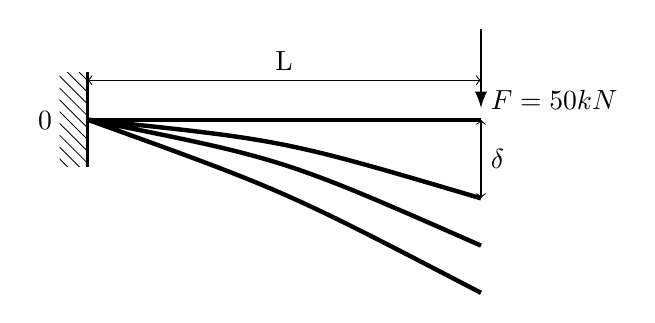
\begin{tikzpicture}
    %the points
    \point{origin}{-0.75}{-0.25};

    \point{begin}{0}{0};
    \point{end}{5}{0};
    \point{end_bot}{5}{-1};
    %the beam
    \beam{2}{begin}{end};
    %the support
    \support{3}{begin}[-90];
    %the load
    \load{1}{end}[90]   ;
    %the inscription of the load
    \notation{1}{origin}{0};
    \notation{1}{end}{$F=50kN$};

     \draw[<->] (end) -- (end_bot) node[midway, right] {$\delta$} ;
     \draw[<->] (0,0.5) -- (5,0.5) node[midway, above] {L};
     
    %the deflection curves
    \draw
      [-, ultra thick] (begin) .. controls (2.5, -.26) .. (5, -1)
      [-, ultra thick] (begin) .. controls (2.5, -.5) .. (5, -1.6)
      [-, ultra thick] (begin) .. controls (2.5, -.9)   .. (5, -2.2);
  \end{tikzpicture}
\label{fig:beam}   
}
%\raggedright
%\hfill
\subfloat[Possible cross-section shapes.]{
\centering

\begin{tikzpicture}
\vspace{1cm}

%%%%%
\tstar{0.25}{0.5}{6}{0}{thick,fill=yellow}
\tstar{0.14}{0.28}{6}{0}{thick,fill=white}

\tstar{0.25}{0.5}{6}{0}{thick,fill=yellow,xshift=-1.2cm}
\tstar{0.08}{0.16}{6}{0}{thick,fill=white,xshift=-1.2cm}

\tstar{0.25}{0.5}{6}{0}{thick,fill=yellow,xshift=-2.4cm}

%%%%%
\def\pos{1.2}
\fill[black] (\pos-0.24,-0.5) -- (\pos-0.24,0.5) -- (\pos+0.24,0.5)  -- (\pos+0.24,-0.5)   -- cycle ;
\fill[black] (\pos-0.5,-0.5) -- (\pos-0.5,-0.18) -- (\pos+0.5,-0.18)  -- (\pos+0.5,-0.5)   -- cycle ; 
\fill[black] (\pos-0.5,0.18) -- (\pos-0.5,0.5) -- (\pos+0.5,0.5)  -- (\pos+0.5,0.18)   -- cycle ;  

\def\pos{2.4}
\fill[black] (\pos-0.19,-0.5) -- (\pos-0.19,0.5) -- (\pos+0.19,0.5)  -- (\pos+0.19,-0.5)   -- cycle ;
\fill[black] (\pos-0.5,-0.5) -- (\pos-0.5,-0.25) -- (\pos+0.5,-0.25)  -- (\pos+0.5,-0.5)   -- cycle ; 
\fill[black] (\pos-0.5,0.25) -- (\pos-0.5,0.5) -- (\pos+0.5,0.5)  -- (\pos+0.5,0.25)   -- cycle ;  

\def\pos{3.6}
\fill[black] (\pos-0.14,-0.5) -- (\pos-0.14,0.5) -- (\pos+0.14,0.5)  -- (\pos+0.14,-0.5)   -- cycle ;
\fill[black] (\pos-0.5,-0.5) -- (\pos-0.5,-0.32) -- (\pos+0.5,-0.32)  -- (\pos+0.5,-0.5)   -- cycle ; 
\fill[black] (\pos-0.5,0.32) -- (\pos-0.5,0.5) -- (\pos+0.5,0.5)  -- (\pos+0.5,0.32)   -- cycle ;  

\vspace{1.2cm}

%%%%%
\fill[green,even odd rule] (0,-1.2) circle (0.5) (0,-1.2) circle (0.33);
\draw (0,-1.2) circle (0.5) ;
\draw (0,-1.2) circle (0.33) 
; 
\fill[green,even odd rule] (-1.2,-1.2) circle (0.5)(-1.2,-1.2) circle (0.17);
\draw (-1.2,-1.2) circle (0.5) ;
\draw (-1.2,-1.2) circle (0.17) 
; 
\fill[green,even odd rule] (-2.4,-1.2) circle (0.5) ;
\draw (-2.4,-1.2) circle (0.5) ;

%%%%%
\def\pos{1.2}
\fill[blue,even odd rule]  (\pos-0.5,-1.7) -- (\pos-0.5,-0.7) -- (\pos+0.5,-0.7) -- (\pos+0.5,-1.7) -- cycle ;

\def\pos{2.4}
\fill[blue,even odd rule]  (\pos-0.5,-1.7) -- (\pos-0.5,-0.7) -- (\pos+0.5,-0.7) -- (\pos+0.5,-1.7) -- cycle   (\pos-0.25,-1.45) -- (\pos-0.25,-0.95) -- (\pos+0.25,-0.95) -- (\pos+0.25,-1.45) -- cycle ;

\def\pos{3.6}
\fill[blue,even odd rule]  (\pos-0.5,-1.7) -- (\pos-0.5,-0.7) -- (\pos+0.5,-0.7) -- (\pos+0.5,-1.7) -- cycle   (\pos-0.35,-1.55) -- (\pos-0.35,-0.85) -- (\pos+0.35,-0.85) -- (\pos+0.35,-1.55) -- cycle ;

  \end{tikzpicture}


\label{fig:beam_shape}    
}
\caption{Cantilever beam problem.}
\end{figure}

Therefore, the problem to model has two continuous variables: the length $L \in [10,20]$ (in $m$) and the surface  $S \in [1,2]$ (in $m^2$) and one categorical variable $ \tilde{I}$ with 12 levels. The tip deflection, at the free end, $\delta$ is given by $$ \delta = f( \tilde{I}, L,S) = \frac{F}{3E} \frac{L^3}{S^2\tilde{I}}. $$

% 98 points
% \begin{table}[H]
% \centering
%  \caption{Results of the cantilever beam models}
% \small

% \resizebox{0.6\columnwidth}{!}{%
% \small

% \begin{tabular}{cccc}
%   method & kernel & RMSE (cm) $\ $   &$\ $ time (s) \\
%   \hline 
%   $mat\_GOWER \ $ & square exponential & 1.386& 6.98     \\   
%   $mat\_CR$ & square exponential & 1.160& 90.98 \\
%   $mat\_EHH$ & square exponential &  &  \\
%   \hdashline 
%   $mat\_GOWER \ $ & absolute exponential &3.240 & 3.02 \\
%   $mat\_CR$ & absolute exponential & 1.980 & 193.60 \\
%   $mat\_EHH$ & absolute exponential &  & \\
% \hline
% \end{tabular}
% }
% \label{tab:resDragon}
% \end{table}
    
To compare our models, we draw a 98 point LHS as training set and the validation set is a grid of $12\times30\times30=10800$ points. For both squared exponential and absolute exponential kernels, the RMSE, likelihood and computational time for every model are shown in~\tabref{tab:resCantilever}. We recall that squared exponential and absolute exponential kernels differ only on the continuous variables and are the same for the categorical part.
As expected, the computational time and the likelihood increase when the model is more complex. The DoE seems of sufficient size for this problem as the computed RMSE (\textit{i.e.}, the total displacement error) decreases with the model complexity.

\begin{table}[H]
\centering
 \caption{Results of the cantilever beam models}
\small

\resizebox{0.9\columnwidth}{!}{%
\small

\begin{tabular}{ccccc}
  Categorical kernel & Continuous kernel & Displacement error (cm) & $ \ $ Likelihood  &$\ $ Time (s) \\
  \hline 
  GD & squared exponential &1.3858 & 111.13&  8.02 \\   
  CR & squared exponential & 1.1604 & 162.26 & 89.1 \\
  EHH & squared exponential &0.1247 &
256.90 & 2769.4 \\
  \hdashline 
  GD & absolute exponential & 3.2403 & 74.48   & 14.71  \\
  CR & absolute exponential & 3.0918 & 99.00 & 260.1 \\
  EHH & absolute exponential & 2.0951& 102.48 & 19784\\
\hline
\end{tabular}
}
\label{tab:resCantilever}
\end{table}

In~\figref{corr_Cantilever}, we have drawn the correlation matrix found between the cross-section shape (the resulting $R_1$ correlation matrix) for the three models. On the figure below, the higher the correlation, the thinner the ellipse. 


\begin{figure}[H]
\begin{center}
	\subfloat[With GD kernel.]{
      \centering 
\includegraphics[clip=true, height=4.6cm, width=5cm]{  Corr_plot_shape23.JPG} \label{corr_canti_gower}
     }  
	\subfloat[ With CR kernel.]{
      \centering
\includegraphics[clip=true, height=4.6cm, width=5cm]{  Corr_plot_shape22.JPG} \label{corr_canti_cr}
     }  
	\subfloat[ With EHH kernel. ]{
      \centering 
\includegraphics[clip=true, height=4.6cm, width=5cm]{  Corr_plot_shape.JPG} \label{corr_canti_ehh}
     }  
\includegraphics[clip=true, height=5cm, width=0.5cm]{  leg.jpg}
\centering     
\caption{Correlation matrix $R_1^{cat}$  using different choices for $\Theta_1$ for the categorical variable $\tilde{I}$ from the cantilever beam problem.}
\label{corr_Cantilever}
\end{center} 
\end{figure}
     
As expected, we have 3 groups of 4 shapes depending on their respective thickness (respectively, the levels \{1,4,7,10\} the levels \{2,5,8,11\} and the levels \{3,6,9,12\}). The more the thickness is similar, the higher the correlation: the thickness has more impact than the shape of the cross-section on the tip deflection. However, given the database, two points with similar $L$ and $S$ values will have similar output whatever the cross-section. The effect of the cross-section on the output is always the same (in the form of $\frac{1}{\tilde{I}}$) leading to an high correlation after maximizing the likelihood. In~\figref{corr_canti_ehh}, with the EHH kernel, we can distinguish the 3 groups of 4 shapes and, because the correlations are close to 1, the homoscedastic hyperphere model~\cite{Pelamatti} would lead to the same correlation matrix.  Also, with the CR kernel of~\figref{corr_canti_cr}, the medium thick group \{2,5,8,11\} being correlated with both the full and the hollow group, its correlation values are the higher whereas the correlation hyperparameters associated to the two other groups are smaller. 
%Hence, CR can retrieve the three groups structure but can not obtain the high in-group correlations as the coefficients associated to both hollow and full group have to be smaller than the ones of the medium group. 
For the GD model in~\figref{corr_canti_gower}, there is only one mean positive correlation value as before.

\subsubsection{Aircraft design application ($n=10$, $ m=0$, $l=2$ and $L_1=9$, $L_2=2$) }
\label{subsec:aircraft}

The ``\texttt{DRAGON}'' aircraft concept %in~\figref{Dragon2020}
has been introduced by ONERA in 2019~\cite{schmollgruber} within the scope of the European CleanSky 2 program\footnote{\href{https://www.cleansky.eu/technology-evaluator}{\color{blue}https://www.cleansky.eu/technology-evaluator}} which sets the objective of 30\% reduction of CO2 emissions by 2035 with respect to 2014 state of the art.
% \begin{figure}[H]
% \begin{center}
%   \begin{subfigure}[b]{.5\linewidth}
%       \centering
% 	\includegraphics[clip=true,height=4cm]{  Dragon2020.pdf}
%       \end{subfigure}
% \end{center}    
%   \begin{subfigure}[b]{.48\linewidth}
%       \centering
% 	\includegraphics[height=5cm]{  onera-dragon-21321165_wagner.jpg}
%       \end{subfigure}~~~
%       %
%       \begin{subfigure}[b]{.48\linewidth}
%       \centering 
% 	\includegraphics[clip=true,height=5cm]{  0246270f-salon-du-bourget-2019-a-quoi-ressemblera-l-avion-du-futur__1200_900__0-418-3891-2612.jpeg}
%   \end{subfigure}
%   \caption{``\texttt{DRAGON}'' aircraft mock-up.}
%         \label{Dragon2020}
% \end{figure}    
The employment of a distributed propulsion comes at a certain cost; a turboelectric propulsive chain is necessary to power the electric fans which brings additional complexity and weight.
%as in~\figref{DragonArchitecture}. 
The turboelectric propulsive chain being an important weight penalty, it is of particular interest to optimize the chain and particularly the number and type of each component, characterized by some discrete values.  The definition of the architecture variable is given in~\tabref{tab:dragon_archi1} and the definition of the turboshaft layout is given in~\tabref{tab:dragon_archi2}. For the sake of simplicity, we restrict the optimization problem to the case of two electric cores and generators but more optimizations have been performed in~\cite{SciTech_cat}.

%
%\begin{figure}[H]
%\vspace*{-0.6cm}
%
%  \centering 
%\includegraphics[clip=true,,height=6cm]{  DragonArchitecture.pdf}
% \caption{Turboelectric propulsive architecture.}
% \label{DragonArchitecture}
%\label{Dragon}
%\end{figure} 

\begin{table}[H]
\centering
\vspace*{-0.1cm}

 \subfloat[Definition of the architecture variable and its 9 associated levels.]{
\small

\resizebox{0.8\columnwidth}{!}{%
\small

\begin{tabular}{cccc}
  Architecture number $\ $ & Number of motors $\ $ & Number of cores $\ $ & Number of generators $\ $ \\
  \hline
  1 & 8 &2 & 2\\
  2 & 12 & 2 & 2\\
  3 & 16 & 2 & 2\\
  4 &20 &2 & 2\\
  5 & 24 & 2 & 2\\
  6 & 28 & 2 & 2\\
  7 &32 & 2 & 2\\
  8 & 36  & 2 & 2\\
  9 & 40 & 2 & 2\\

\hline
\end{tabular}
}
\label{tab:dragon_archi1}
}
\centering
\vspace*{+0.1cm}

\subfloat[Definition of the turboshaft layout variable and its 2 associated levels.]{
\small

\resizebox{0.8\columnwidth}{!}{%
\small

\begin{tabular}{cccccc}
  Layout & Position & y ratio & Tail & VT aspect ratio & VT taper ratio\\
  \hline 
  1 & under wing &0.25 & without T-tail& 1.8 & 0.3 \\
  2 & behind & 0.34 & with T-tail& 1.2 & 0.85\\
 
\hline
\end{tabular}
}
\label{tab:dragon_archi2}
}
\caption{Categorical variable definition}
\end{table}
The analysis of ``\texttt{DRAGON}'' is treated with Overall Aircraft Design method in FAST-OAD~\cite{David_2021}.  We are considering the following problem described in~\tabref{tab:dragon}.
\begin{table}[H]
\centering
\vspace*{-0.3cm}

 \caption{Definition of the ``\texttt{DRAGON}'' optimization problem.}
\small

\resizebox{1.0\columnwidth}{!}{%
\small

\begin{tabular}{lllrr}
 & Function/variable & Nature & Quantity & Range\\
\hline
\hline
Model & Fuel mass & cont & 1 &\\
\hline
with respect to & \mbox{Fan operating pressure ratio} & cont & 1 & $\left[1.05, 1.3\right]$ \\  
     & \mbox{Wing aspect ratio} & cont & 1 &    $\left[8, 12\right]$ \\
    & \mbox{Angle for swept wing} & cont & 1 & $\left[15, 40\right]$  ($^\circ$) \\
     & \mbox{Wing taper ratio} & cont & 1 &    $\left[0.2, 0.5\right]$ \\
     & \mbox{HT aspect ratio} & cont & 1 &    $\left[3, 6\right]$ \\
    & \mbox{Angle for swept HT} & cont & 1 & $\left[20, 40\right]$  ($^\circ$) \\
     & \mbox{HT taper ratio} & cont & 1 &    $\left[0.3, 0.5\right]$ \\
 & \mbox{TOFL for sizing}  & cont &1 & $\left[1800, 2500\right]$ ($m$) \\
 & \mbox{Top of climb vertical speed for sizing $ \ $} & cont & 1 & $\left[300, 800\right]$ ($ft/min$) \\
 & \mbox{Start of climb slope angle} & cont & 1 & $\left[0.075, 0.15\right] $ ($rad$) \\

 & \multicolumn{2}{l}{Total  continuous variables} & 10 & \\
 \cline{2-5}
& \mbox{Architecture} & cat & 9 levels & \{1,2,3, \ldots,7,8,9\} \\
& \mbox{Turboshaft layout} & cat & 2 levels & \{1,2\} \\

 & \multicolumn{2}{l}{Total categorical variables} & 2 & \\
 \cline{2-5}

  &   \multicolumn{2}{l}{\textbf{Total relaxed variables}} & {\textbf{21}} & \\
  \hline

\end{tabular}
}
\label{tab:dragon}
\end{table}

Twice, we draw  $250$ points by LHS. Over the first DoE, that is the training set, we build the model to predict the fuel mass and over the second one, we validate our prediction and compute the RMSE reported in~\tabref{tab:resDragon}.
In this case, the number of hyperparameters is 12 for GD kernel, 21 for CR kernel and 47 for EHH kernel. Evaluating the function is costly, around 4 minutes for a single point. We observed similar performances for all models, the performance is mostly determined by the choice of the continuous kernel. 
For a problem that has that many variables, it seems useless and impractical to use a complicated model, the GD kernel being already performing well. 
On~\figref{corr_turboelectric}, we plot, for the three kernels, the approximate correlation matrices for the first categorical variable. As we can see, when considering the general EHH kernel, as in~\figref{corr_turboelectric_ehh}, the closer the levels, the higher the correlation. In fact, in this case, the only difference between two levels is the number of motors. Therefore, the more similar the number of motors, the more similar the fuel consumption. Given that, we expect, when considering CR kernel as in~\figref{corr_turboelectric_cr} that the higher correlation should appear "in the middle" \{4,5,6\} as these levels are meant to be the most correlated with the others. This is what happens to a certain extent but the levels 7 and 8 are weirdly appearing too much correlated with one another. This could be a numerical problem, the optimization being hard with that many variables and hyperparameters. As before, the GD kernel is the less precise and just give a mean correlation over the whole space as in~\figref{corr_turboelectric_gower}. In~\figref{corr_turboshaft}, we plot, for the three methods, the approximated correlation matrices for the second categorical variable. There is only two engine layouts so there is only one correlation. In this case, the correlation is positive indicating that the plane behave in the same way no matter the layout.


\begin{table}[H]    
\centering
 \caption{Results of the aircraft models based on a 250 point validation set}
\small
\resizebox{0.8\columnwidth}{!}{%
\small

\begin{tabular}{ccccc}
  kernel& $ \ $ number of hyperparameters  & $\ $  kernel   & $\ $fuel error (kg) $\ $  & time (s)   \\
  \hline 
  GD & 12 & squared exponential & 2115 & 65 \\
  CR & 21 & squared exponential & 2068  & 210  \\
  EHH & 47 & squared exponential & 2147 &  9450\\
   \hdashline 
  GD & 12 & absolute exponential &1666 & 65 \\
  CR & 21 & absolute exponential & 1664  & 210 \\
  EHH & 47 & absolute exponential & 1593 &  9295 \\
\hline
\end{tabular}
}
\label{tab:resDragon}
\end{table}



\begin{figure}[H]
\begin{center}
	\subfloat[GD kernel.]{
      \centering 
\includegraphics[clip=true, height=4.4cm, width=5cm]{  Corr_9_archi_gower.JPG} \label{corr_turboelectric_gower}
     }  
	\subfloat[CR kernel.]{
      \centering 
\includegraphics[clip=true, height=4.4cm, width=5cm]{  Corr_9_archi_cr.JPG} \label{corr_turboelectric_cr}
     }  
	\subfloat[EHH kernel.]{
      \centering 
\includegraphics[clip=true,  height=4.4cm, width=5cm]{  Corr_9_archi.JPG}
\label{corr_turboelectric_ehh}
     }  
\includegraphics[clip=true, height=4.7cm, width=0.5cm]{  leg.jpg}
\centering     
\caption{Correlation matrix $R_1^{cat}$  using different choices for $\Theta_1$  for the turboelectric architecture variable.}
\label{corr_turboelectric}
\end{center} 
\end{figure}



\begin{figure}[H]
\begin{center}
\vspace{-1cm}
	\subfloat[GD kernel.]{
      \centering 
\includegraphics[clip=true, height=4.4cm, width=5cm]{  Corr_9_archi2_gower.JPG} \label{corr_turboshaft_gower}
     }  
	\subfloat[CR kernel.]{
      \centering 
\includegraphics[clip=true, height=4.4cm, width=5cm]{  Corr_9_archi2_cr.JPG} \label{corr_turboshaft_cr}
     }  
	\subfloat[EHH kernel.]{
      \centering 
\includegraphics[clip=true, height=4.4cm, width=5cm]{  Corr_9_archi_2.JPG} \label{corr_turboshaft_ehh}
     }  
\centering
\includegraphics[clip=true, height=4.65cm, width=0.5cm]{  leg.jpg}
\caption{Correlation matrix $R_2^{cat}$  using different choices for $\Theta_2$  for the turboshaft layout variable.}
\label{corr_turboshaft}
\end{center} 
\end{figure}

One can note that increasing the number of motors or changing a layout will not change the way an aircraft flies. For example, having more motors will only increase the fuel consumption by a given factor. The latter will always remain positive and related to the continuous variables. Hence, in this test case, we do not have opposite effects between two categorical levels.

In most industrial applications, radically opposite effects over a complex system do not occur so often. For instance, on the industrial applications that can be found on the literature, there was not a clear need for negative correlation values~\cite{Pelamatti,Roustant, cuesta2021comparison}. Therefore, in practice, the exponential model is not that limiting compared to the homoscedastic hypersphere model.  





% \subsubsection{Categorical Branin function}

% Let the function $f$ to model be the modified categorical Branin function~\cite{Gower}. This problem has 3 variables: two continuous variables in $[0,1]$ and one categorical variable with three levels and the two first levels are totally correlated. 
% We draw a DoE of $60$ points by LHS to compare the given GP models and compute the error terms.
% To begin with, we start by plotting the models built with the different methods in~\figref{models_hal5} and compute their respective RMSE to compare them with the original formulation of the methods.
% The obtained values are given in~\figref{models_hal5} from a validation base of size 30603 that corresponds to 101 points from 0 to 1 in every continuous direction for every level (see Appendix~\ref{subsec:branin} for a detailed description of the function).

% \begin{figure}[H]
% \begin{center}
%   \subfloat[Our model (with $\Theta_1=mat\_CR$): RMSE = 60.707]{
%       \centering
% 	\includegraphics[clip=true, height=4cm, width=12cm]{  CP_CR_Hal5.png}} 

% 	\subfloat[Our model (with $\Theta_1=mat\_GOWER$): RMSE = 77.793]{
%       \centering 
% 		\includegraphics[clip=true, height=4cm, width=12cm]{  CP_GOWER_Hal5.png}
%      }  
     
%     % (Homoscedastic hypersphere, RMSE= 63.021
%     \subfloat[Our model (with $\Theta_1=mat\_EHH$): RMSE = 60.721 ]{
%       \centering 
% 	\includegraphics[clip=true, height=4cm, width=12cm]{  CP_HOMO_Hal5.png}}

% 	    \subfloat[Our model (with $\Theta_1=mat\_FULL$): RMSE = 60.707  ]{
%       \centering 
% 		\includegraphics[clip=true, height=4cm, width=12cm]{  /CP_FULL_Hal5.png}
%     }

% \caption{Mean predictions (over the three levels) for the categorical Branin problem using a DoE of 60 points (in red in the curve plots). }\label{models_hal5}
% \end{center} 
% \end{figure}


% In this test case, we clearly show that the full model, the continuous relaxation model and the square exponential homoscedastic one are the same. However, we still have numerical instabilities but using the square exponential homoscedastic kernel as proposed in this paper instead of using the raw matrix leads to a better estimation of the hyperparameters. For homoscedastic hypersphere, the RMSE that we found is 63.021. The Gower distance model is the only one that differs visually and that differs consequently in error from the others (77.8 instead of 60.7). As mentioned in Section~\ref{subsec:hyp_res}, with 3 levels, square exponential homoscedastic hypersphere and continuous relaxation are equivalent methods, so these results were theoretically expected. However, when comparing with the original homoscedastic hypersphere, the square exponential model differs as the third level is negatively correlated from the two others and because the square exponential kernel returns only positive value. In this case, the estimated correlation is 0.03 with the square exponential kernel against -0.15 with the original one. 


%% !TeX spellcheck = en_GB
%!TEX root = ../side-constrained.tex

\section{Conclusion}

We provided a counterexample to a claimed existence result for dynamic equilibria with side constraints. The implications of this counterexample were shown to be severe since solutions to the canonical infinite dimensional variational inequality are in some sense useless and other approaches seem to be necessary. 
We then established a general framework for defining side-constrained dynamic equilibria based on two key objects: A \setS{} $S$ containing all feasible flows (given as walk inflows) and correspondences $A_p$ providing the flow-dependent set of \addmEpsDev s. We showed that this equilibrium concept not only encompasses the known unconstrained equilibria with and without departure time choice and capacitated dynamic equilibria with convex \setS{}s but also allows for a whole range of new dynamic equilibria inspired by static side-constrained equilibria.
We provided conditions under which they can be characterized as solutions to a quasi-variational or even a variational inequality. The latter characterization then also gave rise to a first existence result for certain side-constrained dynamic equilibria with convex \setS.
Finally, we turned to equilibria wherein the side-constraints are given by time-varying edge-load constraints. To deal with the non-convexity of the \setS{}, we employed an augmented Lagrangian approach by relaxing the hard edge-load-capacities and replacing them by penalty functions. We demonstrated that these existence results apply, in particular, for the widely used Vickrey point queue model as well as the linear edge delay model.

Several important questions remain open. First of all, it would be interesting to find an existence result for BSDE similar to \Cref{thm:ExistenceFDAddSpaceExCP} for LPDE and MNSDE. The main obstacle to obtaining such a result seems to be the fact that for BSDE, the definition of \addmEpsDev s involves the network loading which, in general, is a very complex mapping and, even for well-studied flow models, is not fully understood yet. Note that, due to \Cref{prop:RelationshipsOfCDE}, such a result would also directly imply existence of \globalEL{} as well as providing an alternative proof for the existence of LPDE. Another aspect is the multiplicity of equilibria and
the issue of selecting a particular type of equilibrium having desirable properties.
It is an interesting research direction to characterize equilibrium concepts
that admit equilibrium selection via appropriate optimization or optimal control reformulations
whose optimal solutions provide such desirable properties.
\section{Conclusion}
\label{sec:conclu}

In this work, we have proposed a class of kernels for GP models that extends the exponential continuous kernels to the mixed-categorical setting. We showed that this class of kernels generalizes Gower distance and continuous relaxation based kernels. A classification between the proposed kernels as well as a proof of the SPD nature of the resulting correlation matrices have been also proposed. Numerical illustrations on analytical toy problems showed the good potential of the proposed kernels to reduce the number of hyperparameters and thus the computational time. The implementation of our proposed method has been released in the toolbox SMT v2.0\footnote{\url{https://smt.readthedocs.io/en/latest/}}. 
%These GP models are often used for BO, and, as we generalized the continuous relaxation kernel, the previous works that optimized a deep learning model can naturally be extended by our method.  


When considering complex kernels, a good approach would be to use a model reduction technique such as Kriging with Partial Least Squares (KPLS)~\cite{Bouhlel18} that is derived from the construction of the correlation matrix via a kernel function. KPLS is an adaptation of the Partial Least Squares regression for exponential kernels and is used to reduce the number of hyperparameters and handle a large number of mixed inputs. Further works will consider to include such dimension reduction techniques to improve the computational efficiency of our model  and tackle higher dimensional problems. 


\section*{Acknowledgements}
This work is part of the activities of ONERA - ISAE - ENAC joint research group. The research presented in this paper has been performed in the framework of the AGILE 4.0 project (Towards Cyber-physical Collaborative Aircraft Development) and has received funding from the European Union Horizon 2020 Programme under grant agreement n${^\circ}$ 815122. 
We thank Raul Carreira Rufato (ISAE-Supaero MSc) for his contribution to Gower distance implementation, and Dr. Eric Nguyen Van (ONERA) and Christophe David (ONERA) for their contribution to DRAGON aircraft design.
\textcolor{black}{We also thanks the collaborators of SMT, namely ONERA, ISAE-SUPAERO, ICA (CNRS), NASA Glenn, the University of Michigan, Polytechnique Montréal and the University of California San Diego and in particular Rémi Lafage (ONERA).}
The authors are grateful to the partners of the AGILE 4.0 consortium for their contribution and feedback.
%\newpage


%We briefly explain the algebraic background relevant for the definition of the the main character of this paper: the element $A \in \HF(\tau^{-1})$.
We follow the conventions for $A_{\infty}$-machinery from \cite{seidelbook}.

Suppose $\mathcal{A}$ is a homologically unital $A_\infty$-category. The Yoneda embedding is a functor
\[
\mathcal{Y} \colon \mathcal{A} \rightarrow mod_{\mathcal{A}}
\]
taking an object $L$ to the $\mathcal{A}$-module 
$\mathcal{Y}(L)$
defined by
\[
\mathcal{Y}(L)(K) := Mor_{\mathcal{A}}(K,L).
\]
and 
\[
\mu^d_{\mathcal{Y}(L)}(b,a_{d-1}, \dots, a_1) := \mu^d(b, a_{d-1}, \dots , a_1)
\]
for $a_i \in Mor_{\mathcal{A}}(K_{i-1},K_i)$, $i\in \{1, \dots , d-1\}$ 
and $b \in \mathcal{Y}(L)(K_{d-1}) = Mor_{\mathcal{A}}(K_{d-1},L)$.

By \cite[Section 2g]{seidelbook} the Yoneda embedding induces a unital, full and faithfull embedding
\[
\Homol(\mathcal{Y}) \colon \Homol(\mathcal{A}) \to \Homol(mod_{\mathcal{A}}).
\]
The derived cateogory $\mathcal{DA}$ of $\mathcal{A}$
can be constructed as follows: Take a triangulated completion of the image of $\mathcal{Y}$ in $mod_{\mathcal{A}}$ and take its homology category.

The following is an immediate consequence of the properties of the Yoneda embedding. 

\begin{cor}
 Each $f\in Mor_{D\mathcal{A}}(\mathcal{Y}(L_1), \mathcal{Y}(L_2))$ can be represented by 
 $\mathcal{Y}(\alpha)$
 for some $\alpha \in Mor_{\mathcal{A}}(L_1,L_2)$. 
 Moreover, $[\alpha]\in Mor_{H(\mathcal{A})}(L_1,L_2)$ is uniquely defined. 
 \end{cor}
 \begin{proof}
First, note that
\[
Mor_{D\mathcal{A}}(\mathcal{Y}(L_1), \mathcal{Y}(L_2))
\cong \Homol(Mor_{mod_{\mathcal{A}}}(\mathcal{Y}(L_1), \mathcal{Y}(L_2))).
\]
 For any object $K$, $\mathcal{Y}(\alpha)$ determines the map
 \[
 \mathcal{Y}(L_1)(K) \cong Mor(K,L_1) \xrightarrow{\mu^2(\alpha,-)}  
 Mor(K,L_2) \cong \mathcal{Y}(L_2)
 \]
 The existence and uniqueness of $\alpha$ follow immediately from $\Homol(\mathcal{Y})$ being full and faithful.
\end{proof}

\noindent
These notions are applied in this paper to the $A_{\infty}$-category $\mathcal{F}uk(M)$.
 



%%%%%%%%%%%%%%%%%%%%%%%%%%%%%%%%%%%%%%%%%%%%%%%%%%%%%%%%%%%%%%%%%%%%%%%%%%%%
%%%%%%%%%%%Homological Version%%%%%%%%%%%%%%%%%%%%%%%%%%%%%%%%%%%%%%%%%%%%%%
%%%%%%%%%%%%%%%%%%%%%%%%%%%%%%%%%%%%%%%%%%%%%%%%%%%%%%%%%%%%%%%%%%%%%%%%%%%%
\begin{comment}
\subsection{$A_\infty$-categories}
We work in a homological setting, in contrast to Seidel's book.
Moreover, we work in an ungraded setting, maybe later updated to a $\Z / 2\Z$-grading.

We briefly recall here the main definitions and fix notation.

Suppose $\mathcal{A}$ is a homologically unital $A_\infty$-category. The Yoneda embedding is a functor
\[
\mathcal{Y} \colon \mathcal{A} \rightarrow mod_{\mathcal{A}}
\]
taking an object $L$ to the $\mathcal{A}$-module 
$\mathcal{Y}(L)$
defined by
\[
\mathcal{Y}(L)(K) := Mor_{\mathcal{A}}(K,L).
\]
and 
\[
\mu^{\mathcal{Y}(L)}(a_1, \dots, a_{n-1},b) := \mu_n(a_1, \dots , a_{n-1},b)
\]
for $a_i \in Mor_{\mathcal{A}}(K_i,K_{i+1})$, $i\in \{1, \dots , n-1\}$ 
and $b \in \mathcal{Y}(L)(K_n) = Mor_{\mathcal{A}}(K_n,L)$.

By Seidel, section 2g, the Yoneda embedding induces a unital, full and faithfull embedding
\[
H(\mathcal{Y}) \colon H(\mathcal{A}) \to H(mod_{\mathcal{A}}).
\]

The derived cateogory $\mathcal{DA}$ of $\mathcal{A}$
can be constructed as follows: Take a triangulated completion of $mod_{\mathcal{A}}$ and take its homology category.

The following is an immediate consequence of the properties of the Yoneda embedding. We include it here, since it is relevant for this article.

\begin{cor}
 Each $f\in Mor_{D\mathcal{A}}(\mathcal{Y}(L_2), \mathcal{Y}(L_1))$ can be represented by 
 $\mathcal{Y}(\alpha)$
 for some $\alpha \in Mor_{\mathcal{A}}(L_2,L_1)$. 
 Moreover, $[\alpha]\in Mor_{H(\mathcal{A})}(L_2,L_1)$ is uniquely defined. 
 For any object $K$, $\mathcal{Y}(\alpha)$ determines the map
 \[
 \mathcal{Y}(L_2)(K) \cong Mor(K,L_2) \xrightarrow{\mu_2(-,\alpha)}  
 Mor(K,L_1) \cong \mathcal{Y}(L_1)
 \]
 
\end{cor}
\begin{proof}
First, note that
\[
Mor_{D\mathcal{A}}(\mathcal{Y}(L_2), \mathcal{Y}(L_1))
\cong H(Mor_{mod_{\mathcal{A}}}(\mathcal{Y}(L_2), \mathcal{Y}(L_1))).
\]


First, note that
\[
Mor_{D\mathcal{A}}(\mathcal{Y}(L_2), \mathcal{Y}(L_1))
\cong H(Mor_{mod_{\mathcal{A}}}(\mathcal{Y}(L_2), \mathcal{Y}(L_1))) \cong Mor_{H({\mathcal{A}})}(\mathcal{Y}_H(L_2), \mathcal{Y}_H(L_1)),
\]
where $\mathcal{Y}_H(L) = H(Mor_\mathcal{A}(K,L))$.
So $f$ consists of a collection of maps $f(K) \colon Mor_{H(\mathcal{A})}(K,L_2) \to Mor_{H(\mathcal{A})}(K,L_1)$
for every object $K$.

The existence and uniqueness of $\alpha$ follow immediately from $H(\mathcal{Y})$ being full and faithful.
\end{proof}

\end{comment}


%\newpage

%\section{Appendix}
%\appendix

\appendix
\addcontentsline{toc}{section}{Appendix}
\section*{Appendix}

In~\ref{apendix:EHH2CR}, we give the parameterization that allows us to obtain the continuous relaxation kernel using our proposed framework. 
%this appendix describes the two analytical test cases more in details. In Appendix~\ref{subsec:red_blue}, a description of the blue/red case is given and
In~\ref{subsec:cosine}, the cosine test case is detailed. 

\section{Continuous relaxation is a particular instance of our proposed FE Kernel.} 
\label{apendix:EHH2CR}
To show that CR is a particular instance of FE, it suffices to show that the matrix $\Phi(\Theta_i)$ is diagonal whenever $\Theta_i$ is set to a diagonal one. In fact, assume that we have, in our general model, $[\Theta_i]_{j \neq j'} = 0, \  \forall (j,j') \in \{ 1, \ldots, L_i \}.$ 
Knowing that $\cos(0)=1$ and $\sin(0)=0$, the matrix $C(\Theta_i)$ writes as  \\
$$C(\Theta_i) = \begin{bmatrix}
1 & 0 & 0  & 0  \\
1  & 0 &  \ldots & 0 \\
\vdots &\vdots & \ddots & 0 \\
1 &  0 & 0  & 0 \\
\end{bmatrix} \quad \mbox{ and } \quad  C(\Theta_i) C(\Theta_i)^\top = \begin{bmatrix}
1 & 1 & 1  & 1  \\
1  & 1 &  \ldots & 1 \\
\vdots &\vdots & \ddots & 1 \\
1 &  1 & 1  & 1 \\
\end{bmatrix} $$
Therefore, we also have 
$$[\Phi(\Theta_i)]_{j \neq j'} = \frac{\log \epsilon }{2} ([C(\Theta_i) C(\Theta_i)^\top]_{j,j'} -1) = 0, \  \forall (j,j') \in \{ 1, \ldots, L_i \} $$ that is the continuous relaxation kernel. \qed \mbox{}\\ 

% \subsection{2D blue/red test case}
% \label{subsec:red_blue}
% This test case has one categorical variable with two levels: 'blue' or 'red' and one continuous variable in $[0,4]$.
% \begin{itemize}
%     \item The blue DoE of 3 points is the following: x= $\{0,1,4\}$, y=$\{0,9,16\}$
%     \item The red DoE of 4 points is the following: x= $\{0,1,2,3\}$, y=$\{0,1,8,27\}$
% \end{itemize}
% Therefore, we have a DoE consisting of 7 points either blue or red, with continuous value ranging between 0 and 4 and taking value between 0 and 27.



\section{Categorical cosine case}
\label{subsec:cosine}
This test case has one categorical variable with 13 levels and one continuous variable in $[0,1]$~\cite{Roustant}.
Let $w= (x,c )$ be a given point with  $x$ being the continuous variable and $c$ being the categorical variable, $c \in \{1, \ldots, 13\}$.

\begin{equation*}
\begin{split}
f(w) &= \cos \left( \frac{7 \pi}{2} x + \left( 0.4 \pi  + \frac{\pi }{15} c  \right) - \frac{c}{20} \right) , ~~~\mbox{if c $\in\{10,\ldots,9\}$ }  \\
f(w) &= \cos \left( \frac{7 \pi}{2} x  - \frac{c}{20} \right) , ~~~\mbox{if c $\in\{10,\ldots,13\}$ }  \\
\end{split}
\end{equation*}
The reference landscapes of the objective function (with respect to the categorical choices) are drawn on~\figref{fig:Roustant_ref}.

\begin{figure}[H]
\centering
\includegraphics[scale=.12]{  Roustant_curves.png}
\caption{Landscape of the cosine test case from~\cite{Roustant}.}
\label{fig:Roustant_ref}    
\end{figure}    
The DoE is given by a LHS of 98 points.
% Our DoE drawn by LHS is the following: 
% $x= \left\{ \vphantom{[]^2}\right.$[ 0.65605253,  6.        ],
%       [ 0.83350264,  4.        ],
%       [ 0.15026485,  7.        ],
%       [ 0.24143059, 12.        ],
%       [ 0.03096315,  8.        ],
%       [ 0.23260394,  9.        ],
%       [ 0.21316332, 11.        ],
%       [ 0.80211976,  4.        ],
%       [ 0.94950991,  1.        ],
%       [ 0.58874134,  2.        ],
%       [ 0.15866055,  8.        ],
%       [ 0.29988981,  4.        ],
%       [ 0.11186171,  4.        ],
%       [ 0.3476918 ,  2.        ],
%       [ 0.01205944,  3.        ],
%       [ 0.71141884,  8.        ],
%       [ 0.28951039,  5.        ],
%       [ 0.73724151,  9.        ],
%       [ 0.38762527,  0.        ],
%       [ 0.3443474 ,  1.        ],
%       [ 0.31419979,  0.        ],
%       [ 0.97505473,  0.        ],
%       [ 0.71769637, 11.        ],
%       [ 0.14208871,  9.        ],
%       [ 0.02645321, 11.        ],
%       [ 0.64144679,  4.        ],
%       [ 0.93347456,  1.        ],
%       [ 0.26023608,  4.        ],
%       [ 0.36179242, 11.        ],
%       [ 0.19235854,  3.        ],
%       [ 0.82539539, 12.        ],
%       [ 0.77423165,  1.        ],
%       [ 0.62454224,  5.        ],
%       [ 0.56235338,  4.        ],
%       [ 0.68487501, 12.        ],
%       [ 0.52396804,  6.        ],
%       [ 0.31718476,  9.        ],
%       [ 0.49061463,  6.        ],
%       [ 0.69566705,  2.        ],
%       [ 0.60557496,  2.        ],
%       [ 0.90013372,  2.        ],
%       [ 0.77980976,  2.        ],
%       [ 0.99262069,  6.        ],
%       [ 0.61237851,  9.        ],
%       [ 0.07168795,  2.        ],
%       [ 0.37433399,  3.        ],
%       [ 0.51563867,  7.        ],
%       [ 0.06439778,  6.        ],
%       [ 0.39792487, 10.        ],
%       [ 0.09111936,  2.        ],
%       [ 0.54844499, 10.        ],
%       [ 0.6778083 ,  0.        ],
%       [ 0.10018382,  3.        ],
%       [ 0.78794137,  0.        ],
%       [ 0.48618283,  0.        ],
%       [ 0.64305827,  7.        ],
%       [ 0.98717047,  4.        ],
%       [ 0.92111218, 11.        ],
%       [ 0.9095025 ,  5.        ],
%       [ 0.42987802, 10.        ],
%       [ 0.5931088 ,  6.        ],
%       [ 0.57328161,  7.        ],
%       [ 0.85035836, 11.        ],
%       [ 0.04171931,  5.        ],
%       [ 0.96455513, 11.        ],
%       [ 0.05890046,  2.        ],
%       [ 0.28382111,  2.        ],
%       [ 0.81016573,  5.        ],
%       [ 0.00382184,  7.        ],
%       [ 0.8454141 ,  8.        ],
%       [ 0.93911432,  8.        ],
%       [ 0.66928872, 11.        ],
%       [ 0.12230256, 11.        ],
%       [ 0.20098996,  6.        ],
%       [ 0.25362715,  7.        ],
%       [ 0.75857015,  4.        ],
%       [ 0.18005584,  8.        ],
%       [ 0.55734768, 11.        ],
%       [ 0.44058174,  7.        ],
%       [ 0.21558225,  3.        ],
%       [ 0.88253717,  3.        ],
%       [ 0.42716698, 12.        ],
%       [ 0.7281732 ,  0.        ],
%       [ 0.27491291,  7.        ],
%       [ 0.16597145,  8.        ],
%       [ 0.86510046,  2.        ],
%       [ 0.46646275, 12.        ],
%       [ 0.39911793,  9.        ],
%       [ 0.12286505,  1.        ],
%       [ 0.33037   ,  1.        ],
%       [ 0.86803419,  6.        ],
%       [ 0.47060982, 12.        ],
%       [ 0.44960284,  4.        ],
%       [ 0.89443379,  3.        ],
%       [ 0.53266967,  5.        ],
%       [ 0.41534775,  6.        ],
%       [ 0.50583278,  0.        ],
%       [ 0.75433057, 10.        ]$\left.\vphantom{[]^2}\right\}$
Our validation set is a evenly spaced grid of 1000 points in $x$ ranging  for every of the 13 categorical levels  for a total of 13000 points.



%\nocite{*}
%\bibliography{sample}

\bibliographystyle{elsarticle-num-names} 
\bibliography{main}
%%%%%%%%%%%%%%%%%%%%%%%%%%%%%%%%%%%%%%%%%%%%%%%%%%%%%%%%%%%%%%%%%%%%%%

\end{document}